\chapter{Diseño e implementación} % Main chapter title

\label{Chapter3} % Change X to a consecutive number; for referencing this chapter elsewhere, use \ref{ChapterX}

\definecolor{mygreen}{rgb}{0,0.6,0}
\definecolor{mygray}{rgb}{0.5,0.5,0.5}
\definecolor{mymauve}{rgb}{0.58,0,0.82}

%%%%%%%%%%%%%%%%%%%%%%%%%%%%%%%%%%%%%%%%%%%%%%%%%%%%%%%%%%%%%%%%%%%%%%%%%%%%%
% parámetros para configurar el formato del código en los entornos lstlisting
%%%%%%%%%%%%%%%%%%%%%%%%%%%%%%%%%%%%%%%%%%%%%%%%%%%%%%%%%%%%%%%%%%%%%%%%%%%%%
\lstset{ %
  backgroundcolor=\color{white},   % choose the background color; you must add \usepackage{color} or \usepackage{xcolor}
  basicstyle=\footnotesize,        % the size of the fonts that are used for the code
  breakatwhitespace=false,         % sets if automatic breaks should only happen at whitespace
  breaklines=true,                 % sets automatic line breaking
  captionpos=b,                    % sets the caption-position to bottom
  commentstyle=\color{mygreen},    % comment style
  deletekeywords={...},            % if you want to delete keywords from the given language
  %escapeinside={\%*}{*)},          % if you want to add LaTeX within your code
  %extendedchars=true,              % lets you use non-ASCII characters; for 8-bits encodings only, does not work with UTF-8
  %frame=single,	                % adds a frame around the code
  keepspaces=true,                 % keeps spaces in text, useful for keeping indentation of code (possibly needs columns=flexible)
  keywordstyle=\color{blue},       % keyword style
  language=[ANSI]C,                % the language of the code
  %otherkeywords={*,...},           % if you want to add more keywords to the set
  numbers=left,                    % where to put the line-numbers; possible values are (none, left, right)
  numbersep=5pt,                   % how far the line-numbers are from the code
  numberstyle=\tiny\color{mygray}, % the style that is used for the line-numbers
  rulecolor=\color{black},         % if not set, the frame-color may be changed on line-breaks within not-black text (e.g. comments (green here))
  showspaces=false,                % show spaces everywhere adding particular underscores; it overrides 'showstringspaces'
  showstringspaces=false,          % underline spaces within strings only
  showtabs=false,                  % show tabs within strings adding particular underscores
  stepnumber=1,                    % the step between two line-numbers. If it's 1, each line will be numbered
  stringstyle=\color{mymauve},     % string literal style
  tabsize=2,	                   % sets default tabsize to 2 spaces
  title=\lstname,                  % show the filename of files included with \lstinputlisting; also try caption instead of title
  morecomment=[s]{/*}{*/}
}

En este capítulo se detalla el diseño de la arquitectura del sistema en todos sus componentes. Se menciona el motivo de elección en cada caso y la implementación correspondiente.

%----------------------------------------------------------------------------------------
%	SECTION 1
%----------------------------------------------------------------------------------------
\section{Diseño de la estructura general del sistema}
\label{seccion-intro}
La estructura del sistema implementado puede observarse en la figura \ref{fig:esquema-general}. El sistema consta de clientes que serán navegadores web para acceder al frontend y a las API \citep{WEBSITE:34} que contiene el backend. Por otro lado, del lado del cliente, los dispositivos conversores Modbus a MQTT se conectan al broker que también forma parte del servidor.

Las funciones implementadas en el backend se conectan a una base de datos remota para almacenar los datos de clientes web o bien mediciones de dispositivos conectados.

\begin{figure}[htpb]
	\centering
	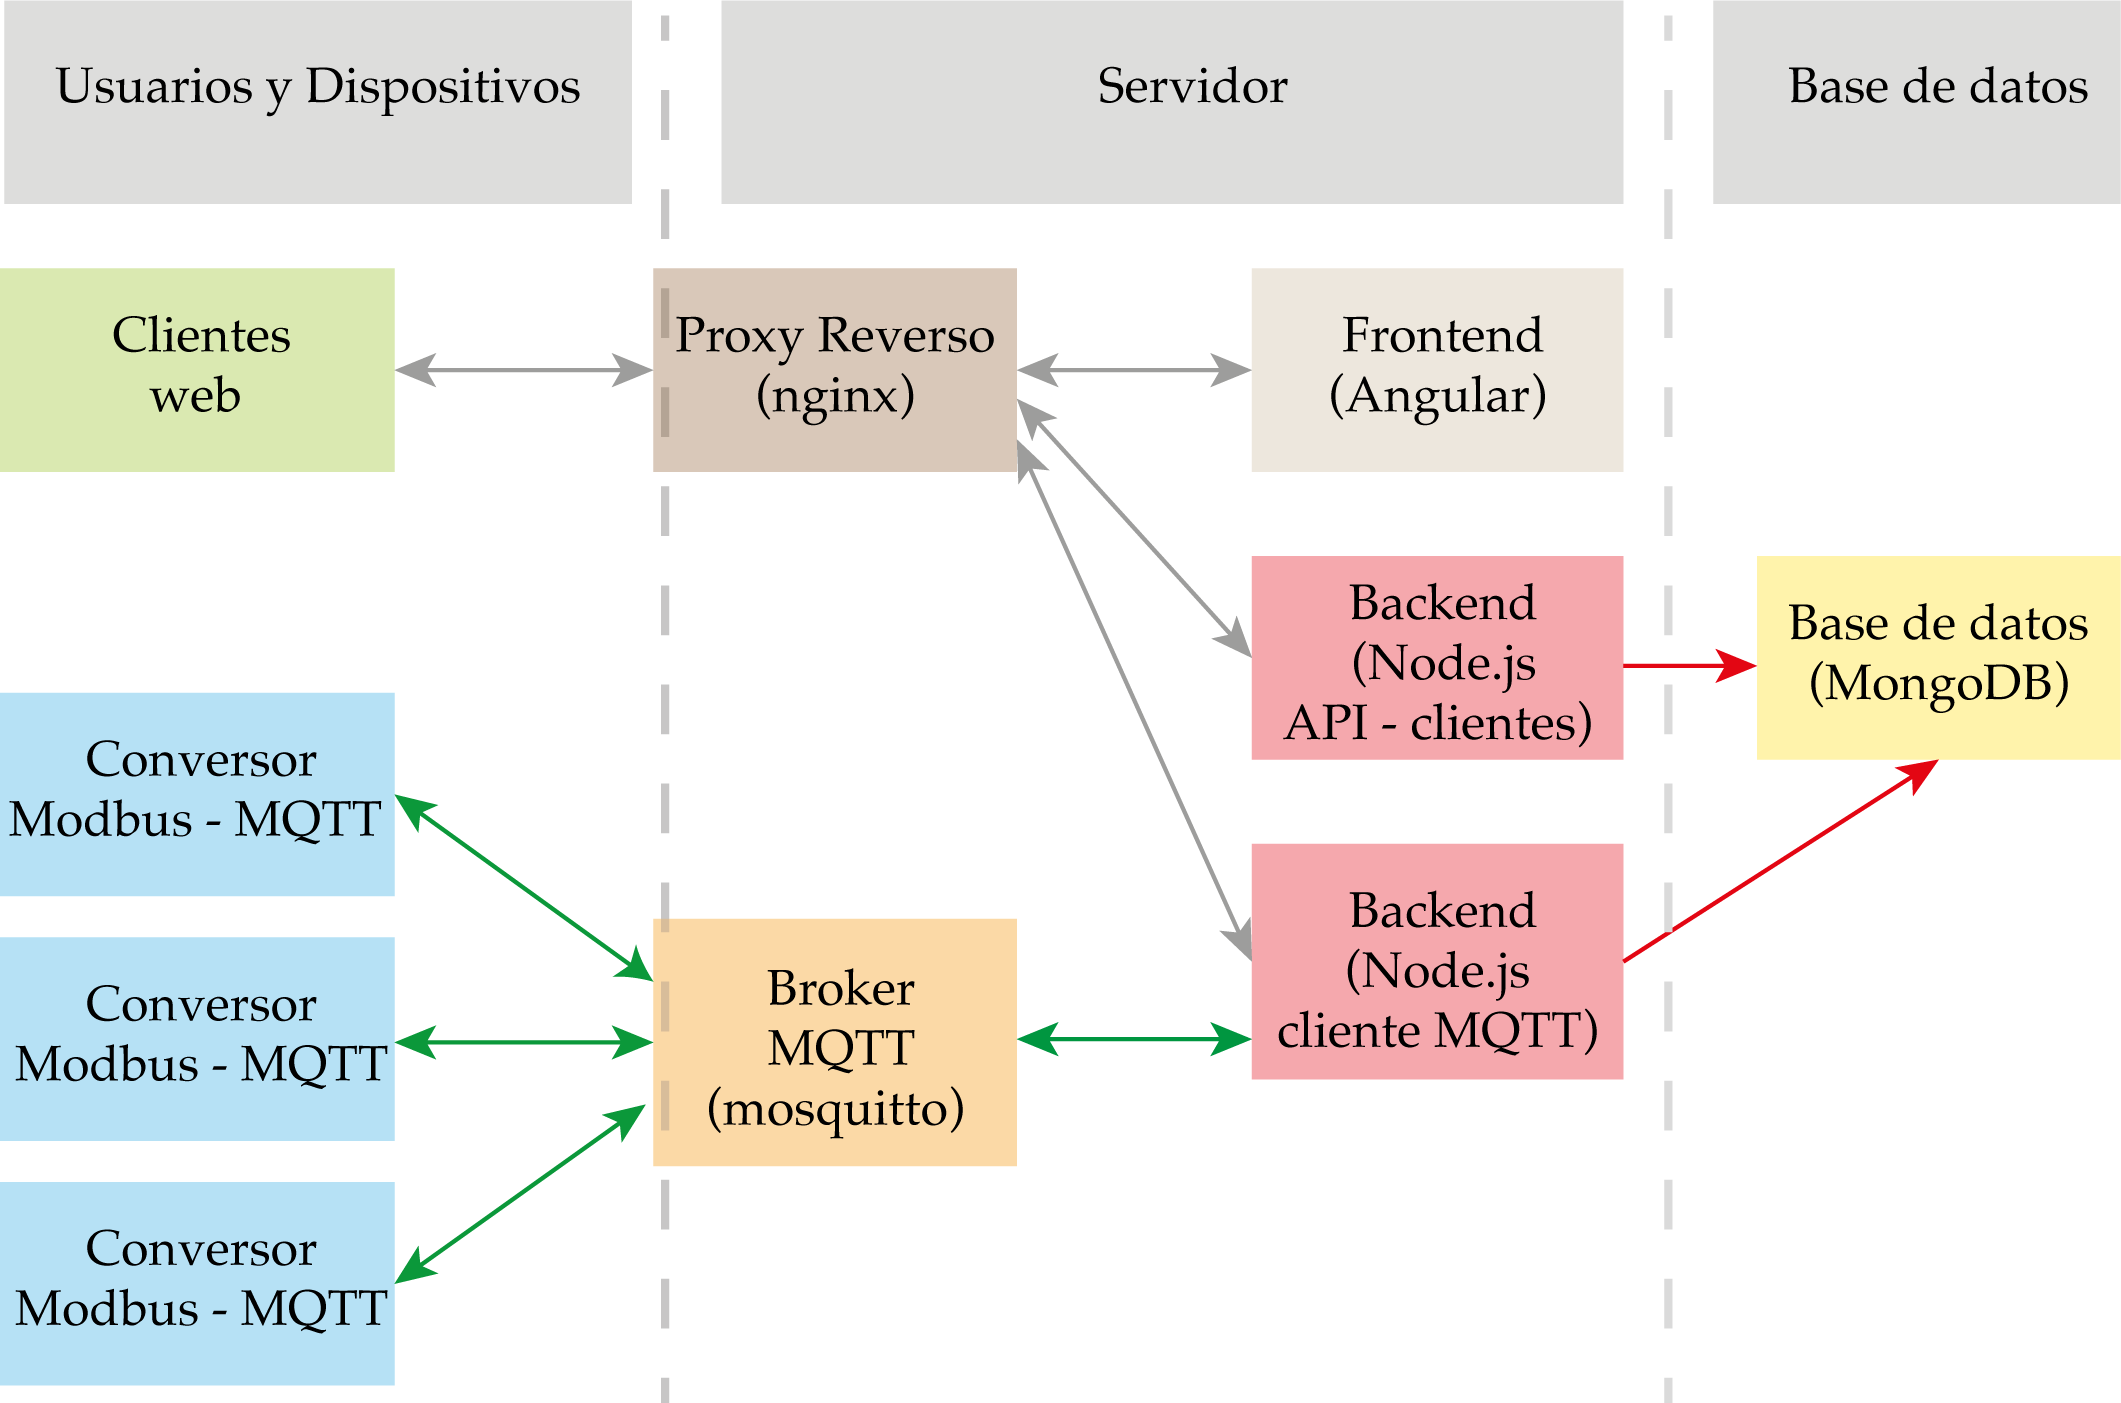
\includegraphics[scale=.75]{./Figures/esquema-general.png}
	\caption[Diagrama de bloques de sistema implementado ]{Diagrama de bloques de sistema de gestión implementado.}
	\label{fig:esquema-general}
\end{figure}
 
En el servidor se desarrolló el frontend en Angular mientras que el backend consta de dos módulos. Por un lado el modulo de API de clientes que fue desarrollado en Node.js y contiene la implementación de funciones para interactuar con la base de datos y la creación de usuarios, dispositivos y visualización de configuración.  Además, el backend consta de un módulo cliente MQTT que se encarga de interactuar entre el broker y los dispositivos conectados a él. Es el encargado de gestionar la información que envían los dispositivos hacia la base de datos para luego ser utilizados por el frontend. 

Todo el servidor es gestionado por Nginx, el cual actúa como proxy inverso lo que permite un único canal de comunicación entre usuarios y sistema.  Por último, la base de datos se encuentra en un servidor remoto y se accede a ella mediante credenciales de conexión. 
 
 
\section{Implementación del backend}
\label{backend-sec}
El backend del trabajo realizado está divido en diferentes bloques de funcionamiento. 

El bloque de backend de funciones API de clientes que se observa en la figura \ref{fig:backend-clientes} donde su conexión con el punto de entrada al servidor gestionado por Nginx es el puerto 8000.  Por otro lado, este bloque se conecta con la base de datos remota MongoDB Atlas \citep{WEBSITE:35} para almacenar datos de nuevos usuarios, dispositivos, configuración de dispositivos, organizaciones y relaciones entre usuarios y organizaciones.  Los clientes que acceden a cualquier función de este bloque lo harán a través de un puerto seguro, dotado de certificados SSL que es manejado por Nginx y mapeado al puerto 8000.

\begin{figure}[htpb]
	\centering
	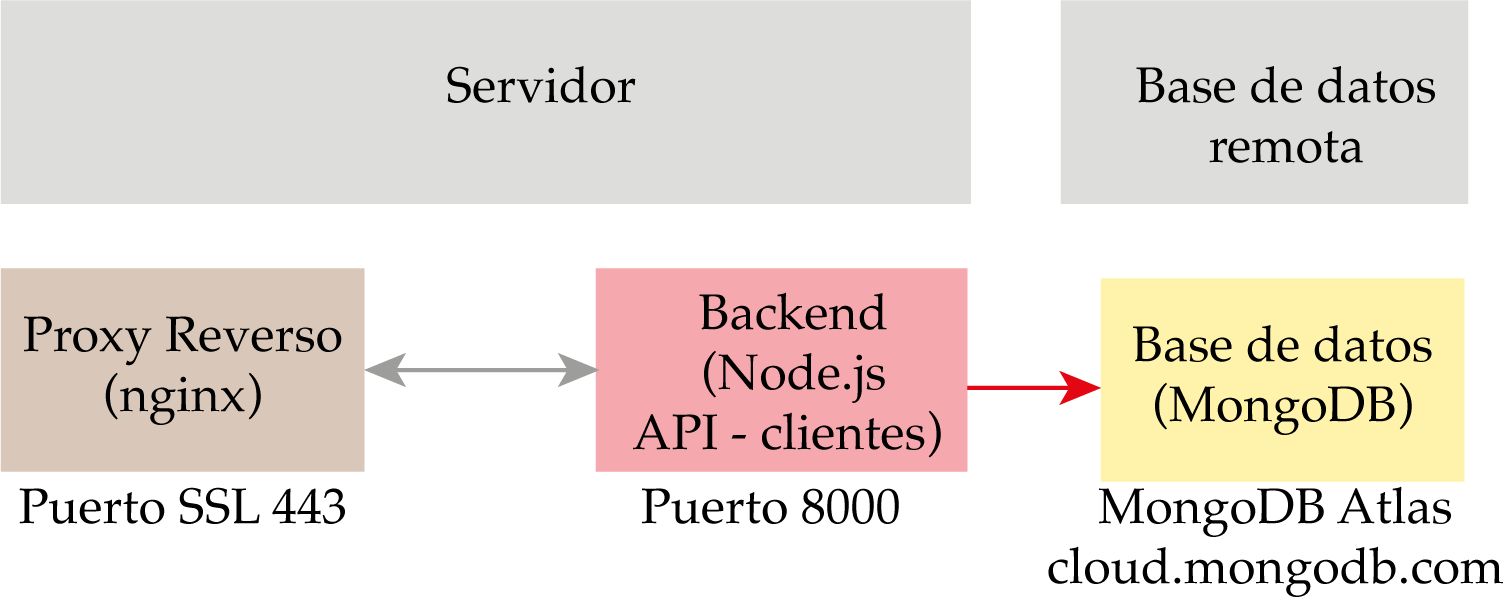
\includegraphics[scale=.75]{./Figures/backend-clientes.png}
	\caption[Conexión entre Nginx - API clientes y base de datos]{Diagrama de conexión entre Nginx, modulo de API de clientes y base de datos en MongoDB Atlas.}
	\label{fig:backend-clientes}
\end{figure}

La estructura interna de este bloque consta de rutas y un bloque de funciones para el manejo antes mencionado. En la figura \ref{fig:bloque-api-clientes} puede observarse un desglose general de este bloque. 

\begin{figure}[htpb]
	\centering
	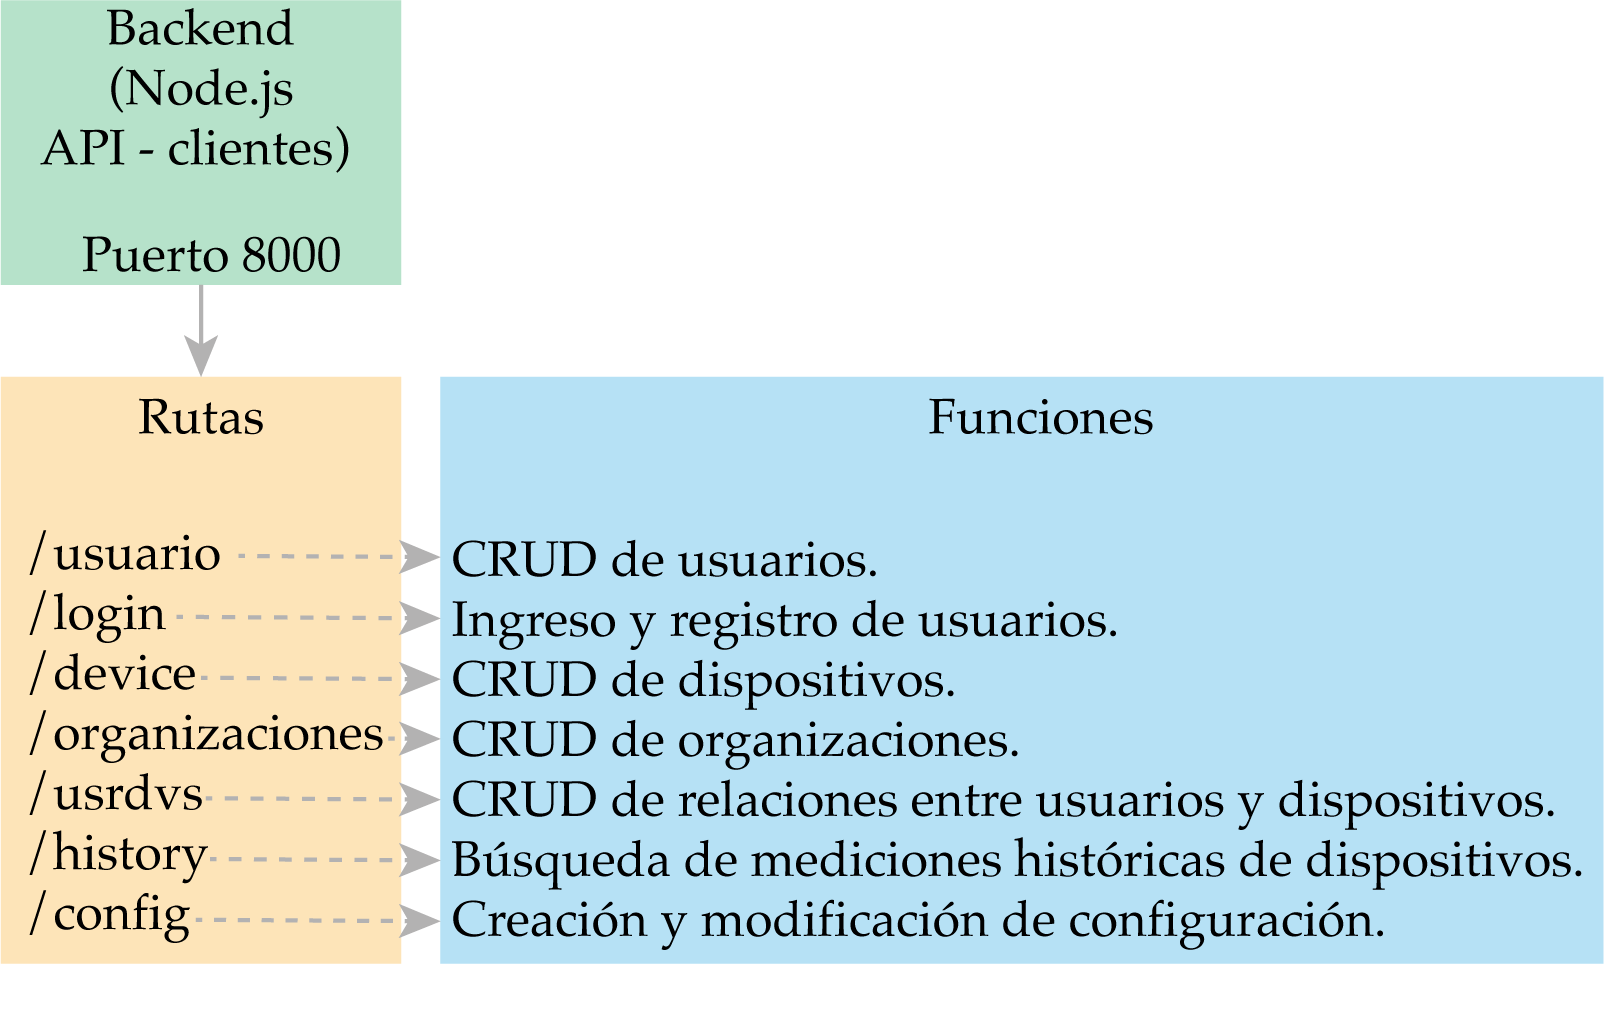
\includegraphics[scale=.75]{./Figures/bloque-api-clientes.png}
	\caption[Descripción bloque API clientes]{Descripción de rutas y funciones principales de bloque API clientes.}
	\label{fig:bloque-api-clientes}
\end{figure}

Se utilizó la librería de Node.js llamada Express.js \citep{WEBSITE:36} la cual proporciona mecanismos para:

\begin{itemize}
	\item Escritura de manejadores de peticiones con diferentes verbos HTTP en diferentes rutas.
	
	\item Integración con motores de renderización de vistas para generar respuestas mediante la introducción de datos en plantillas.
	
	\item Establecer ajustes de aplicaciones web como qué puerto usar para conectar, y la localización de las plantillas que se utilizan para renderizar la respuesta.

	\item Añadir procesamiento de peticiones \textit{middleware} adicional en cualquier punto dentro de la tubería de manejo de la petición.

\end{itemize}

En el código \ref{cod:express-code} se muestra la forma adoptada para crear las rutas para las funciones de gestión.

\begin{lstlisting}[label=cod:express-code,caption=Utilización de Express para crear rutas en el servidor.] 

// Inclusion del modulo express

var express = require('express');

var app = express();

//Rutas 
app.use('/usuario', require('./routes/usuario'));

app.use('/login', require('./routes/auth'));

app.use('/device', require('./routes/devices'));

app.use('/organizaciones', require('./routes/organizations'));

app.use('/usrdvs', require('./routes/usrs_dev'));

app.use('/history', require('./routes/historical'));

app.use('/config', require('./routes/sensors-config'));


// Escuchar peticiones
app.listen(process.env.PORT, () => {
    console.log('server: \x1b[32m%s\x1b[0m', 'running');
});

\end{lstlisting}

Otra biblioteca importante que se utiliza en este bloque es Mongoose \citep{WEBSITE:38}, que se utiliza para escribir consultas para una base de datos de MongoDB, con características como validaciones, construcción de \textit{queries, middlewares,} conversión de tipos entre otras, que enriquecen la funcionalidad de la base de datos. 

La parte central del uso de Mongoose está en la definición de un esquema donde se indica la configuración de los documentos para una colección de MongoDB.  En el código \ref{cod:mongoose-code} se muestra su inicialización y la conexión remota. 

\begin{lstlisting}[label=cod:mongoose-code,caption=Utilización de Mongoose para el manejo de MongoDB.] 

// Inclusion de mongoose.
var mongoose = require('mongoose');

// Conexion a la base de dato remota
try {
        await mongoose.connect( process.env.DB_CNN , {
            useNewUrlParser: true, 
            useUnifiedTopology: true,
            useCreateIndex: true
        });

        console.log('DB Online');
        
    } catch (error) {
        console.log(error);
        throw new Error('Error a la hora de iniciar la BD');
    }
}

\end{lstlisting}


Además, dentro del backend del trabajo realizado, se encuentra el bloque para el manejo de mensajes MQTT que se publican en el broker y provienen de los dispositivos conectados a él.  En la figura \ref{fig:backend-mqtt-server} se puede ver su conexión con el broker y además con la base de datos MongoDB. 

\begin{figure}[htpb]
	\centering
	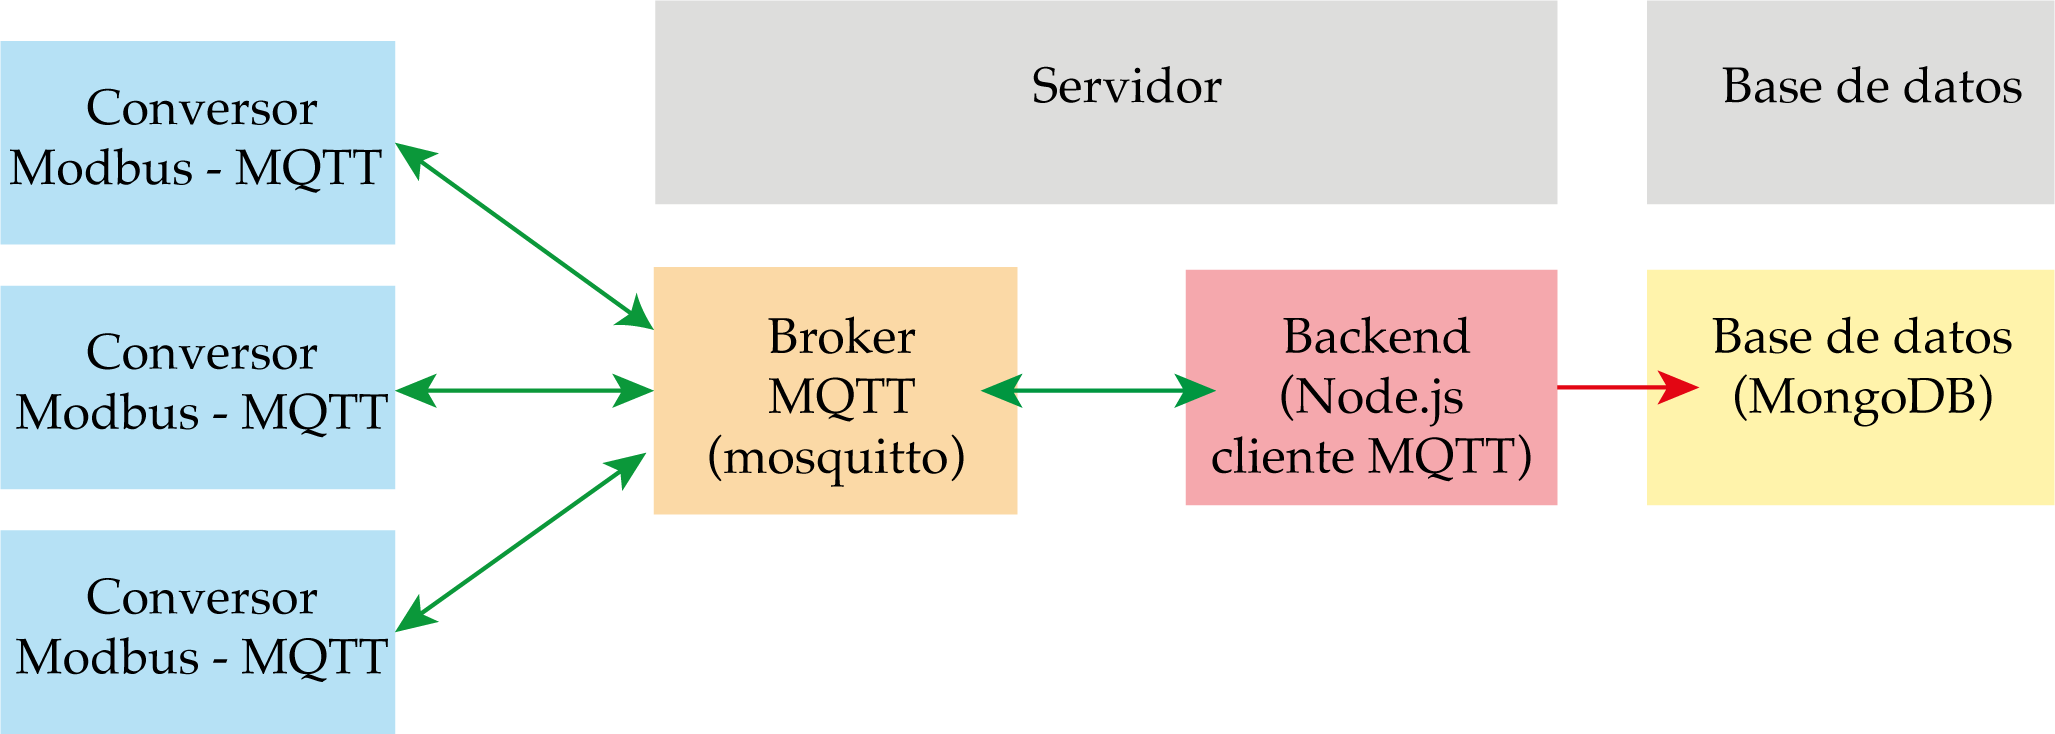
\includegraphics[scale=.75]{./Figures/backend-mqtt.png}
	\caption[Descripción bloque cliente MQTT]{Descripción de cliente MQTT implementado en el servidor.}
	\label{fig:backend-mqtt-server}
\end{figure}


Para crear un cliente MQTT en Node.js se utiliza la librería MQTT.js \citep{WEBSITE:38} con la cual se pueden crear clientes que se conecten al broker del sistema. En el código \ref{cod:mqtt-code} se muestra la implementación en el backend del servidor.

\begin{lstlisting}[label=cod:mqtt-code,caption=Cliente MQTT en el servidor utilizando librería  MQTT.js.] 

// Incluimos la libreria mqtt
var mqtt = require('mqtt');

// Definicion de variables de conexion.
var options= {
            port: +process.env.MB_PORT,
            username: process.env.MB_USERNAME,
            password: process.env.MB_PASSWORD,           
};
   
// Conexion al broker MQTT     
var client  = mqtt.connect(process.env.MB_URL, options);

/* Evento de conexion con el broker */
client.on('connect', function() {
		logger._log('info','MQTT broker conectado');

            /* Subscripcion a los topicos */
           MQTTsubscriber.subscribe(client);
});

/* Evento de error en la conexion con el broker */
client.on('error', (error) => {
        	logger._log('error','Error: ' + error.message);
            
});

/* Evento de reconexion del broker */
client.on('reconnect', () => {
		logger._log('warn','Reconectando al Broker MQTT');
});

/* Evento de conexion cerrada con el broker */
client.on('close', () => {
		logger._log('warn','Conexion con el broker cerrada');
});

/* Evento de broker Offline */
client.on('offline', () => {
		logger._log('info','Conexion con el broker Offline');
});

/* Evento de broker finalizado */
client.on('end', () => {
	 	logger._log('info','Conexion con el broker Finalizada');
});

/* Evento de mensaje del broker donde se recibe 
* el topico y el mensaje 
*/
client.on('message', function(topic, message, packet) {
	 	console.log(topic);
		console.log(message);
	 	console.log(packet);

		MQTTsubscriber.observe(topic,message,packet);
});
\end{lstlisting}


\subsection{Modelos utilizados en la base de datos}

Para el manejo de la base de datos, Mongoose requiere que se creen \textit{Schemas} de cada uno de los modelos que intervienen en este trabajo. 

Para la implementación del modelo de usuario se realizó un estudio de los campos que serán utilizados por el cliente para el registro y acceso al sistema. El código  \ref{cod:user-model}  muestra esta definición en conjunto con sentencias para validar información del modelo.

\begin{lstlisting}[label=cod:user-model,caption=Definición de Schema para el modelo de usuario.] 

// Inclusion de librerias utilizadas
var mongoose = require('mongoose');
var uniqueValidator = require('mongoose-unique-validator');

// Definicion de Schema
var Schema = mongoose.Schema;

// Variable con roles permitidos cuando se crea un usuario.
var rolesValidos = {
    values: ['CREATOR_ROLE', 'ADMIN_ROLE', 'USER_ROLE'],
    default: 'USER_ROLE',
    message: '{VALUE} no es un rol permitido'
};

//Creo el schema para el modelo de Usuario
var usuarioSchema = new Schema({

    nombre: { type: String, required: [true, 'El nombre es requerdio'] },
    email: { type: String, unique: true, required: [true, 'El correo es necesario'] },
    
    role: { type: String, 
            required: true, 
            default: 'USER_ROLE', 
            enum: rolesValidos },
    created_by: { type: Schema.Types.ObjectId, ref: 'Usuario', require:[true, 'debe crearlo un usuario'] },
    created: { type: String, default: '' },
    updated: { type: String, default: '' },
    deleted: { type: String, default: '' },
});

// Plugin que me permite enviar un mensaje de error cuando se hacen las validaciones.
usuarioSchema.plugin(uniqueValidator, { message: '{PATH} debe ser unico' });

// Exporto el modelo para que se pueda utilizar en las funciones del programa.
module.exports = mongoose.model('Usuario', usuarioSchema);

\end{lstlisting}

Para el resto de los modelos utilizados en el trabajo, el procedimiento adoptado es similar al del código \ref{cod:user-model}. En la figura \ref{fig:modelos-mongo} se muestran los modelos más utilizados en este trabajo para realizar operaciones con la base de datos. 

\begin{figure}[htpb]
	\centering
	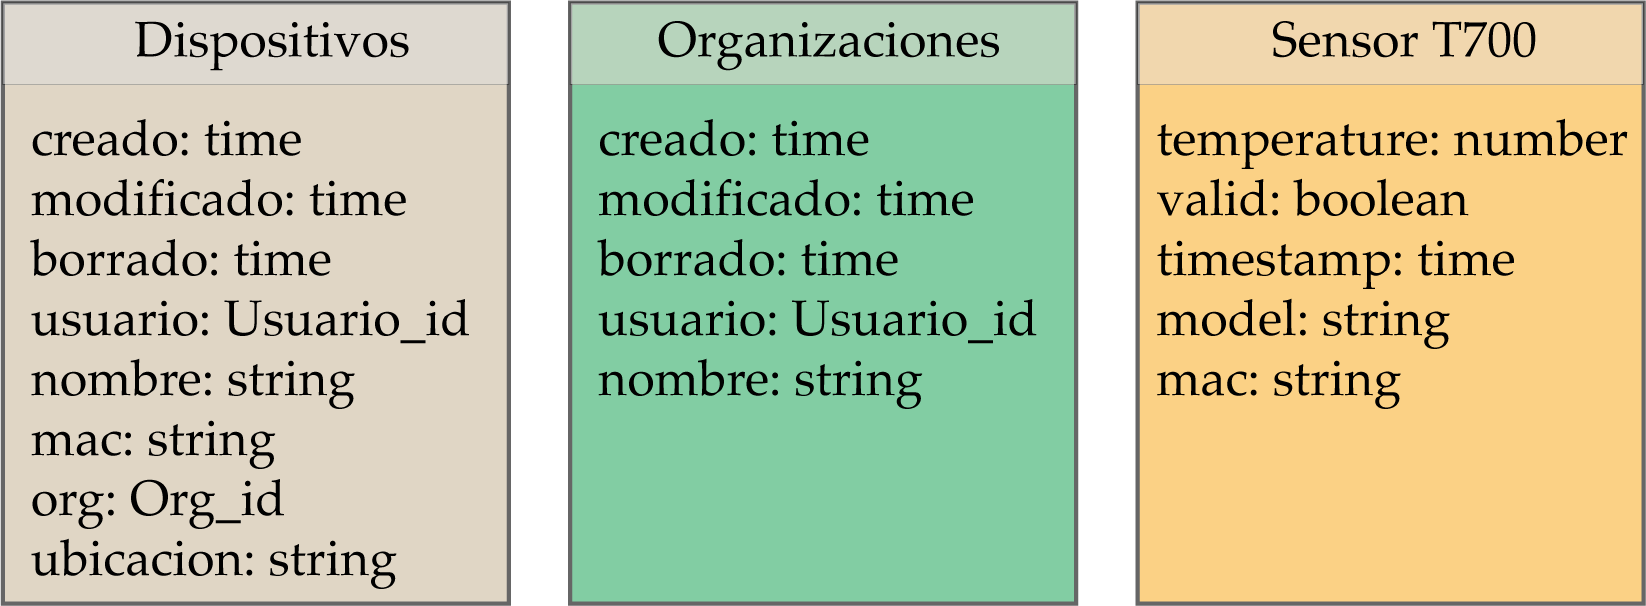
\includegraphics[scale=.75]{./Figures/modelos-mongo.png}
	\caption[Modelos de datos utilizados en Mongoose]{Descripción modelos de datos utilizados para crear los Schemas para realizar operaciones en Mongoose.}
	\label{fig:modelos-mongo}
\end{figure}


\subsection{Implementación CRUD para el manejo de usuarios }

Como se mencionó en la sección \ref{backend-sec}, en el bloque del backend encargado de manejar las funciones APIs para crear nuevos usuarios y dispositivos, entre otras funcionalidades, se implementaron funciones para crear, modificar, leer y borrar cada uno de ellos. Además, se implementaron criterios de búsqueda de dispositivos y usuarios teniendo en cuenta parámetros que provienen de las rutas. 

\begin{lstlisting}[label=cod:crud-usuario,caption=Implementación CRUD para usuarios que se registran.] 

/* Crear un nuevo usuario*/

const crearUsuario = async (req, res = response) => {
    const { nombre, email, password, role, created_by} = req.body;  
/* Completo los campos del modelo*/
        var usuario = new Usuario({
            nombre: nombre,
            email: email,
            role: role,
            created_by: created_by,
            created: new Date().toISOString(),      
        });
/* Guardo el nuevo usuario en la base de datos*/
        await usuario.save();
        /* Envio la respuesta*/
        res.json({
            ok: true,
            usuario
        });   
}

/* Borrar un usuario*/
const borrarUsuario = async (req, res = response) => {
    const id = req.params.id;
        await Usuario.findByIdAndDelete( id );
        res.json({
            ok: true,
            msg: 'Usuario Eliminado'
        })
}

/* Leer un usuario*/
const getUsuarioById = async (req, res = response) => {
    var id = req.params.id;
        const user = await Usuario.findById(id)
                        .populate('nombre email role password')
        res.status(200).json({
            ok: true,
            usuario: user
        });
}

/* Editar un usuario*/
const actualizarUsuario = async (req, res = response) => {
    var id = req.params.id;
    const { password, email, role, ...campos} = req.body;

    campos.updated = new Date().toISOString();
    const usuarioActualizado = await Usuario.findByIdAndUpdate( id, campos, {new: true});
        res.json({
            ok: true,
            usuario: usuarioActualizado
        })
}

\end{lstlisting}


Para la implementación del CRUD de organizaciones y dispositivos, se empleó el mismo concepto de programación, utilizando los modelos correspondientes. 


\subsection{Configuración del broker MQTT}
\label{mqtt-sec}

El broker MQTT utilizado para este trabajo es Mosquitto \citep{WEBSITE:39}. Es un servidor de mensajes de código abierto (con licencia EPL/EDL) que implementa las versiones 3.1 y 3.1.1 del protocolo MQTT. Es ampliamente utilizado debido a su rapidez, lo que permite emplearlo en gran número de ambientes, incluso si éstos son de pocos recursos. En la sección \ref{mqtt-section} se explicó en detalle el uso del protocolo MQTT y se especificó el funcionamiento del broker. 

La configuración de Mosquitto se realiza a través de un archivo interno que se encuentra entre los archivos de instalación del broker con el nombre de \textit{mosquitto.conf}. 

En el código \ref{cod:broker-conf} se muestra el uso y aplicación de cada parámetro configurado para este trabajo. 

\begin{lstlisting}[label=cod:broker-conf,caption=Configuración utilizada en Mosquitto como broker MQTT.] 

/* Comando para no permitir conexiones de usuarios anonimos*/
allow_anonymous false

/* Defino que el password se guardara en la carpeta passwd*/
password_file /etc/mosquitto/passwd

/* Conexion en el puerto 1883 para los dispositivos - sin seguridad */
listener 1883

/* Conexion en el puerto 884 con aplicacion de seguridad SSL */
listener 884

/* Utilizacion de protocolo MQTT por websockets para este puerto*/
protocol websockets

/* Utilizacion de protocolo MQTT por websockets para este puerto*/
certfile /
cafile /
keyfile /

\end{lstlisting}

\subsection{Seguridad en el servidor}

Para dotar de seguridad al servidor, se instalaron certificados SSL que es un estándar de seguridad global que permite la transferencia de datos cifrados entre un navegador y un servidor web.

Para establecer esta conexión segura, se instala en un servidor web un certificado SSL (también llamado certificado digital) que cumple dos funciones:

\begin{itemize}
	\item Autenticar la identidad del sitio web, garantizando a los visitantes que no están en un sitio falso.
	
	\item Cifrar la información transmitida.

\end{itemize}

Para dotar de seguridad al sistema se utilizó una herramienta llamada \textit{certbot} \citep{WEBSITE:40} y en el código \ref{cod:certificados-ssl} se muestran los pasos realizados para instalar los certificados en Nginx.

\begin{lstlisting}[label=cod:certificados-ssl,caption=Procedimiento realizado para instalar certificados SSL en Nginx.] 

// Habilitar https a traves del firewall
sudo ufw allow 'Nginx Full'
sudo ufw delete allow 'Nginx HTTP'

/* Obtener un certificado SSL para el dominio utilizado en este trabajo*/

sudo certbot --nginx -d cloud.dytsoluciones.com.ar -d www.cloud.dytsoluciones.com.ar

/* Se completan los pasos requeridos por Certbot y para verificar la instalacion se ejecuta el comando*/

sudo systemctl status certbot.timer

/* Ademas, para testea el proceso de renovacion se ejecuta*/
sudo certbot renew --dry-run

\end{lstlisting} 

Una vez realizados estos pasos, el acceso al servidor sera por HTTPS y el sitio estará protegido.

\section{Implementación del frontend}

Para el diseño del frontend, se tuvo en cuenta los siguientes requerimientos:

\begin{itemize}
	\item Debe ser un cliente del broker MQTT para poder observar datos en tiempo real de los dispositivos conectados.
	
	\item Debe tener funciones de consultas hacia la base de datos a través del backend. 
	
	\item Debe contar con un menú de configuración para vinculación de nuevos dispositivos. 
	
	\item Debe adaptarse a cualquier tamaño de pantalla como ser celulares, tabletas y monitores.
	
	\item Debe tener acceso protegido con usuario y contraseña para cada usuario. 

\end{itemize}


Para la implementación se utilizó Angular como \textit{framework} de programación.


\subsection{Diseño de plataforma web con Angular}

La estructura general de la plataforma consta de una pantalla de inicio donde el usuario puede iniciar sesión, o bien realizar un registro al sistema para luego poder ingresar al sistema. 

En la figura \ref{fig:pantalla-login} se pueden observar la pantalla de login, mientras que la figura \ref{fig:pantalla-register} muestra la pantalla de registro de usuario. 

\begin{figure}[htpb]
	\centering
	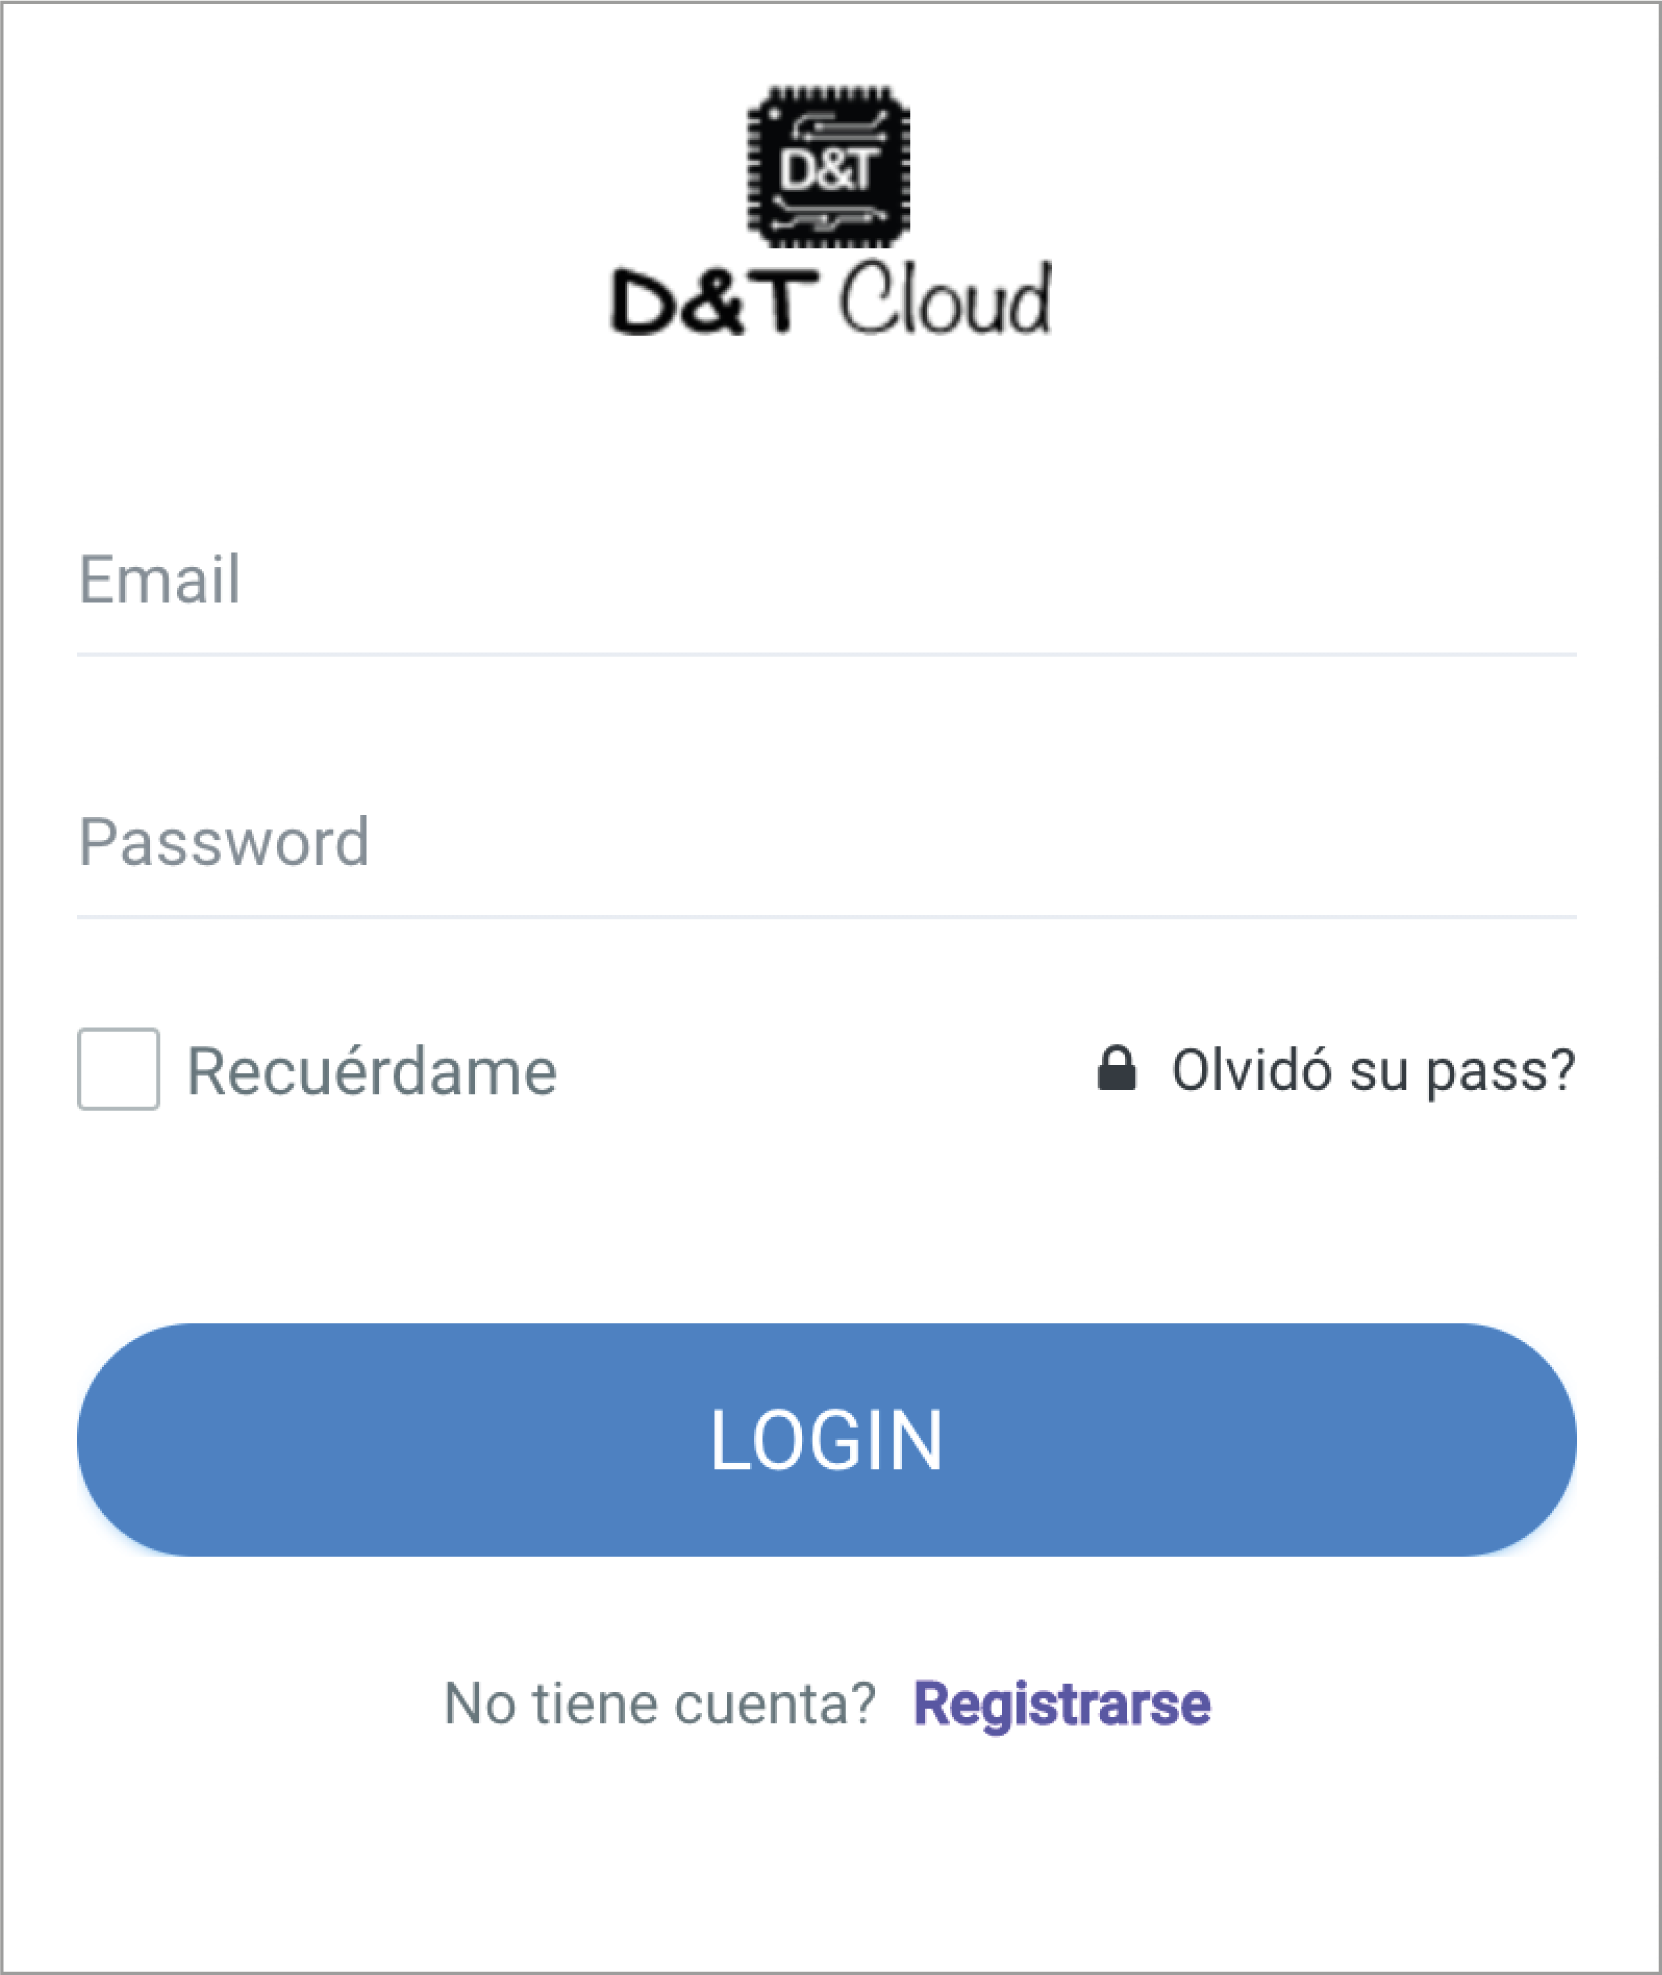
\includegraphics[scale=.60]{./Figures/pantalla-login.png}
	\caption[Pantalla de login de usuario]{Ilustración de pantalla de login de usuario en plataforma web.}
	\label{fig:pantalla-login}
\end{figure}
\pagebreak
\begin{figure}[htpb]
	\centering
	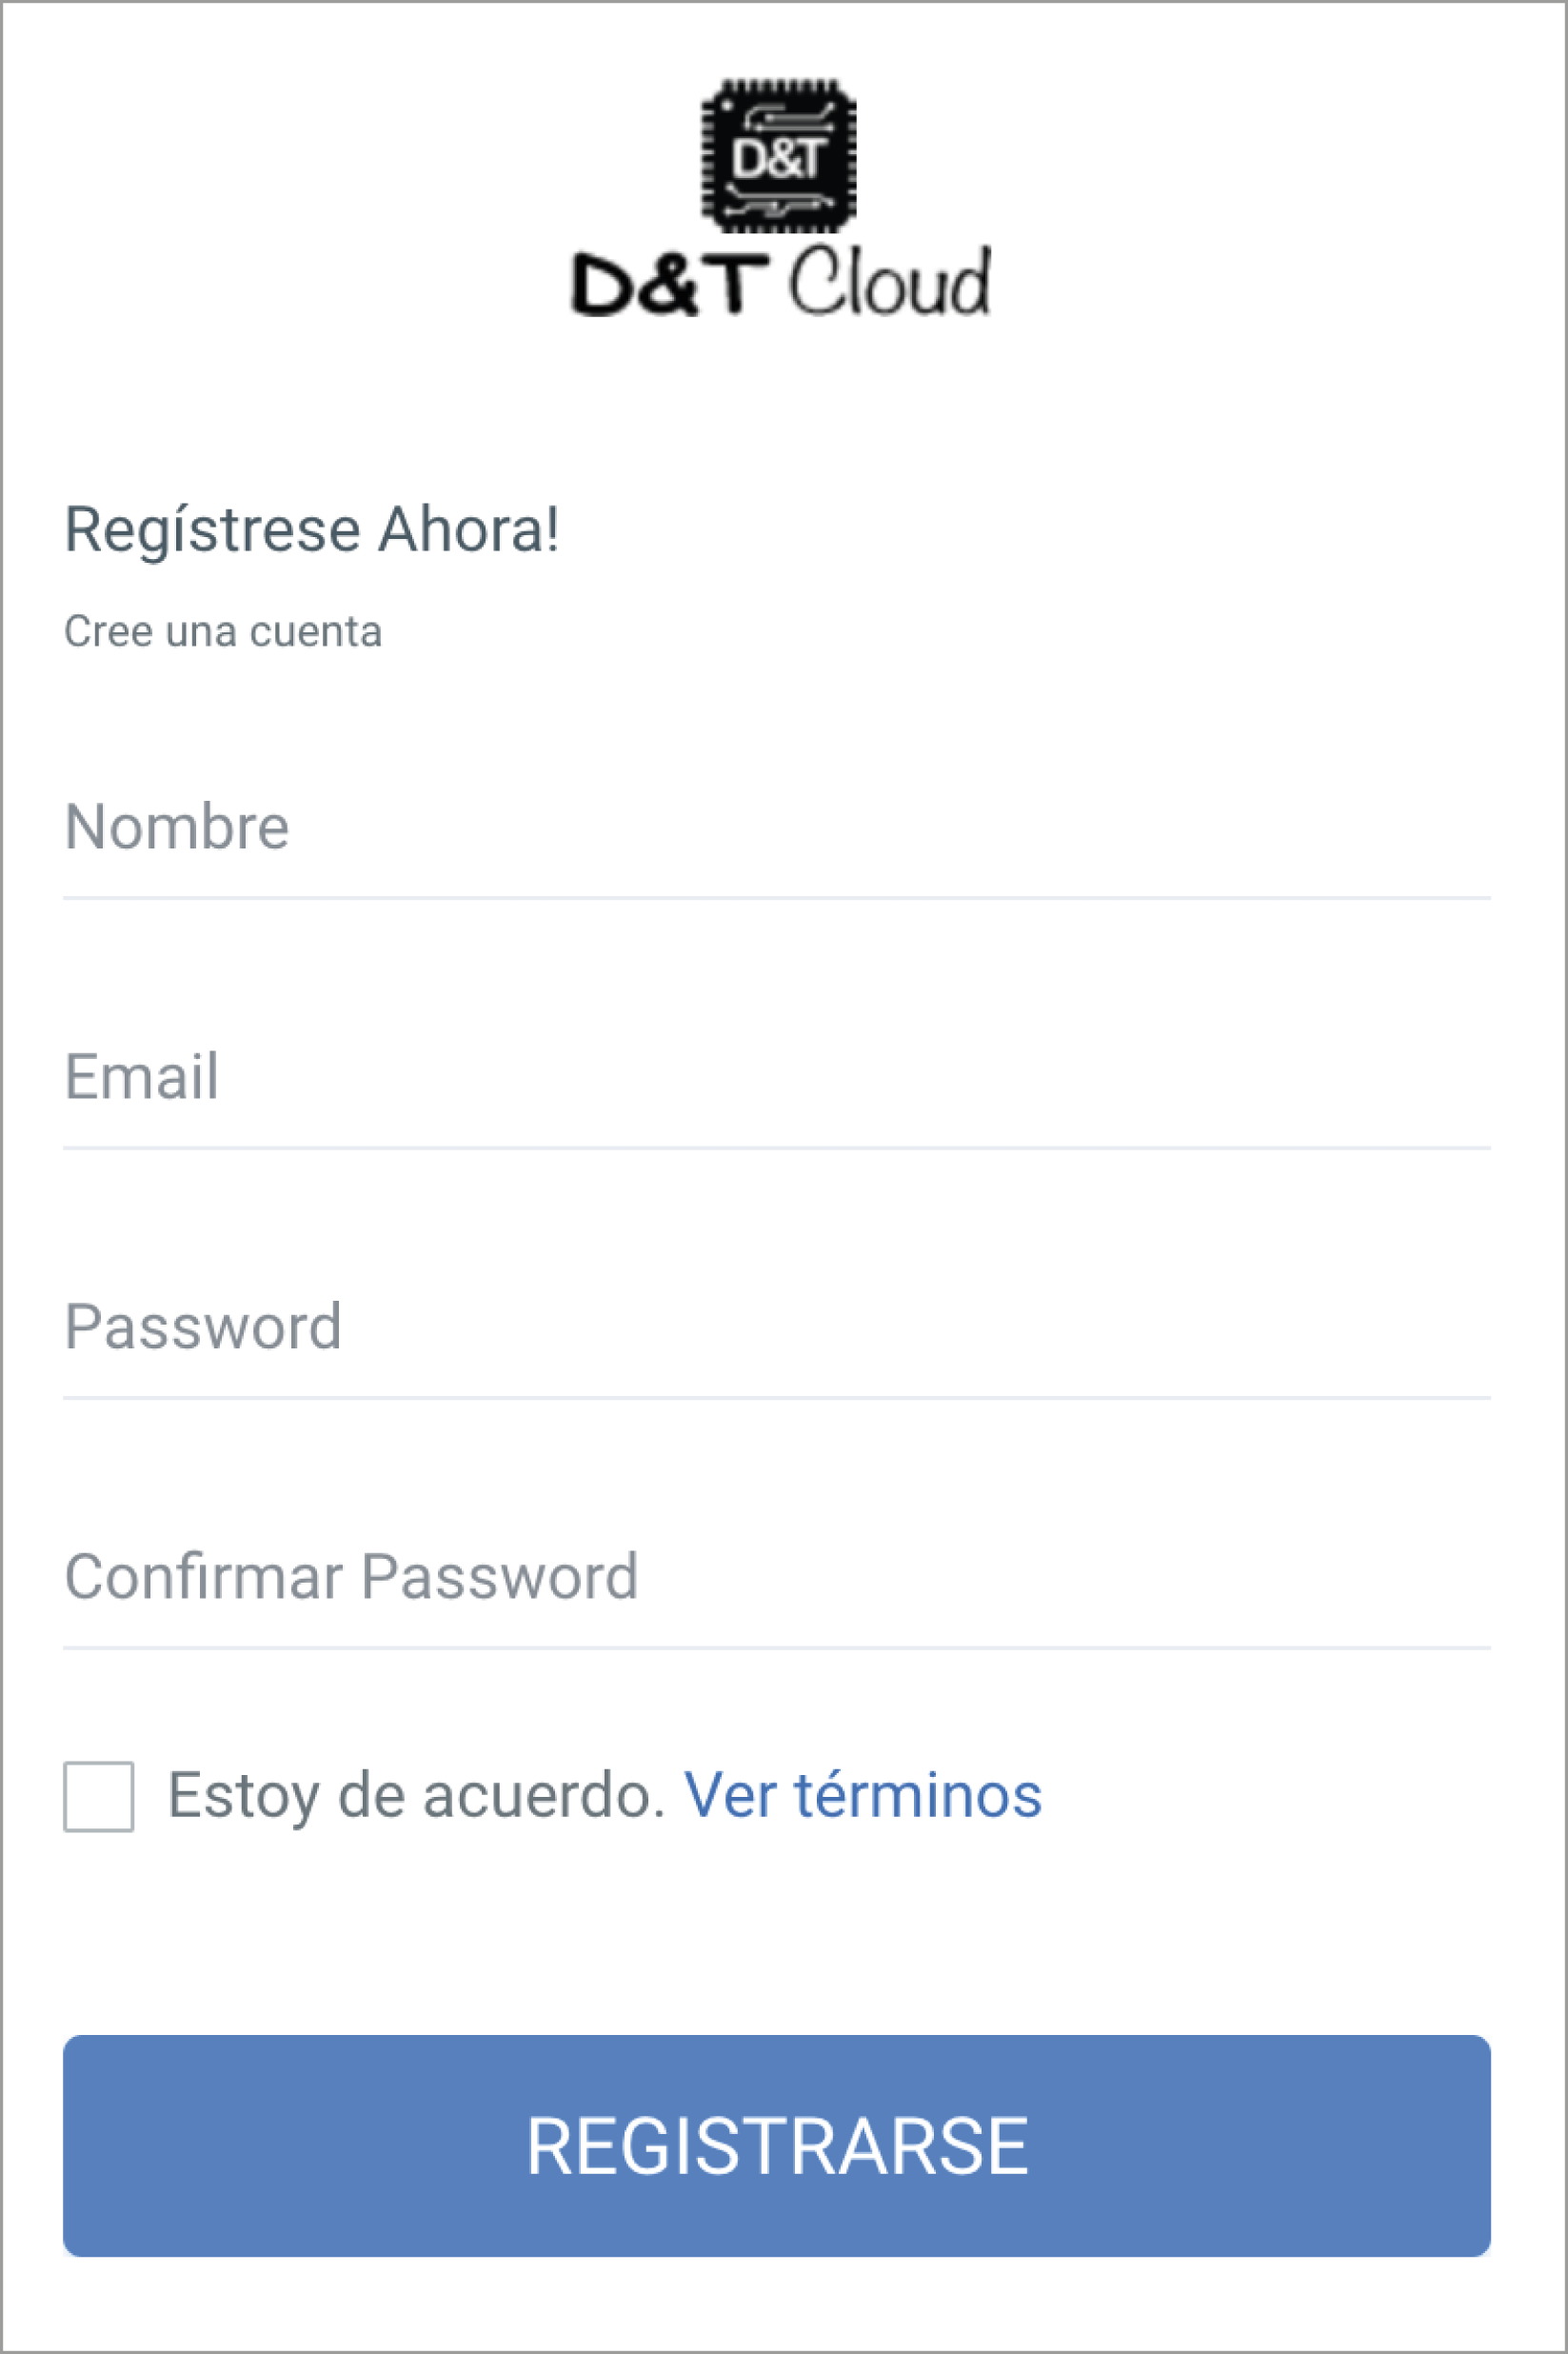
\includegraphics[scale=.60]{./Figures/pantalla-register.png}
	\caption[Pantalla de registro de usuario]{Ilustración de pantalla de registro de usuarios en plataforma web.}
	\label{fig:pantalla-register}
\end{figure}


Para la implementación en Angular, dentro de la carpeta /src se creo un componente para la pantalla de login y un componente para la pantalla de registro. En la figura \ref{fig:estructura-login} puede observarse la estructura y archivos creados para el desarrollo de las pantallas antes mencionadas. 

\begin{figure}[htpb]
	\centering
	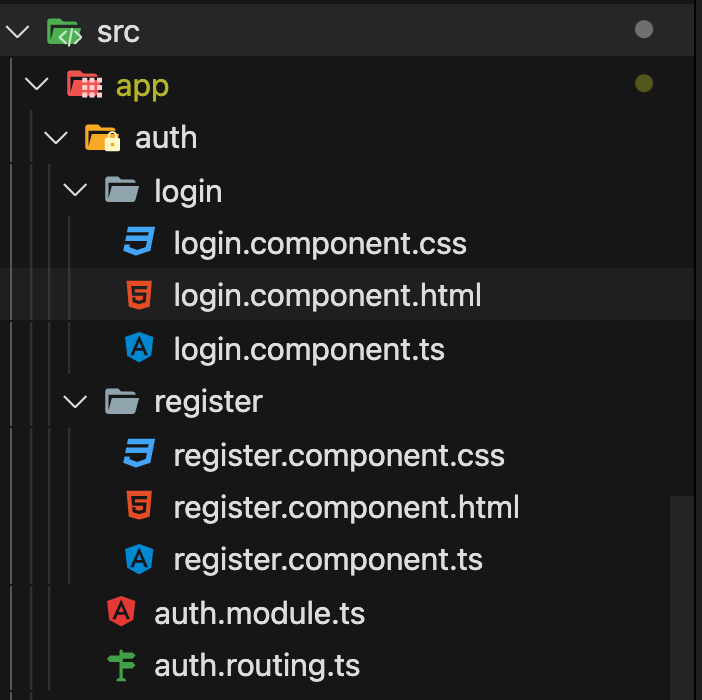
\includegraphics[scale=.50]{./Figures/estructura-login-vs.png}
	\caption[Estructura de componentes de login y registro]{Ilustración de estructura creada en el desarrollo de la pantalla de login y registro.}
	\label{fig:estructura-login}
\end{figure}

\pagebreak

Los comandos de angular utilizados para crear estos componentes se pueden observar en el código \ref{cod:crear-componentes}.

\begin{lstlisting}[label=cod:crear-componentes,caption=Comandos de Angular para crear componentes de login y registro.] 

// Comando para crear el componente login en la carpeta auth
ng create component auth/login
// Comando para crear el componente register en la carpeta auth
ng create component auth/register

\end{lstlisting} 

Para la programación del componente login, se utilizó una plantilla HTML para formar la imagen deseada y utilizar dos campos de texto para introducir el usuario y contraseña.  En el código \ref{cod:html-login}. se puede observar la implementación de los aspectos principales de la pantalla teniendo en cuenta que además se utilizaron clases CSS para asignarle el estilo deseado. 

\begin{lstlisting}[label=cod:html-login,caption=Desarrollo de código HTML para la pantalla de login teniendo en cuenta estilos de diseño CSS.] 

<div class="card-body">

            <form (submit)="login()" 
                 class="form-horizontal form-material" 
                 id="loginform"
                 autocomplete="off"
                 [formGroup]= "loginForm">
               
                <div class="form-group m-t-40">
                    <div class="col-xs-12">
                        <input class="form-control" 
                            type="email" 
                            placeholder="Email"
                            formControlName='email'
                            >
                    </div>
                </div>
                <div class="form-group">
                    <div class="col-xs-12">
                        <input class="form-control" 
                                type="password"
                                placeholder="Password"
                                formControlName='password'>
                    </div>
                </div>
                
                <div class="form-group text-center m-t-20">
                    <div class="col-xs-12">
                        <button class="btn btn-info btn-lg btn-block text-uppercase btn-rounded" 
                            type="submit"
                            [class.spinner]="isLoading" [disabled]="isLoading">Log In</button>
                    </div>
                </div>
                      
            </form>
        </div>


\end{lstlisting} 

Otro aspecto importante en el desarrollo de la pantalla es la programación del comportamiento de cada campo en el que el usuario interactúa con la página. El código \ref{cod:ts-login} muestra las funciones principales que se programaron en el archivo \textit{Typescript}.

\begin{lstlisting}[label=cod:ts-login,caption=Fragmentos de código más relevantes utilizado en el archivo \textit{Typescript} del componente login.] 

// Definicion de clase LoginComponent
export class LoginComponent {

  public formSubmitted = false;
  public isLoading = false;

  public loginForm = this.fb.group({  
    email:[localStorage.getItem('email') || '', [Validators.required, Validators.email]],
    password: ['', Validators.required],
    remember: [false]
  });

// Constructor de la clase donde se incluyen servicios para utilizar
  constructor(private router:Router,
              private fb: FormBuilder,
              private usuarioService: UsuarioService,
              private sweetAlert:SweetAlertService
              ) { }
              
// Metodo login(), cuando el usuario presiona el boton
  login(){
    this.formSubmitted = true;
    this.isLoading = true;
    if(this.loginForm.invalid){
      this.isLoading = false;
      return;
    }
// Validacion del formulario 
    if (this.loginForm.get('remember').value){
      localStorage.setItem('email',this.loginForm.get('email').value)
    }else{
      localStorage.removeItem('email');
    }
// Utilizacion de servicio inyectado en el constructor.
    this.usuarioService.loginUsuario(this.loginForm.value)
      .subscribe(resp => {
        console.log('login correcto', resp);
        this.isLoading = false;
// Si el login es correcto, navega a la pagina principal. 
        this.router.navigateByUrl('/');
      },
      (err) => {
        console.log(err);
        this.isLoading = false;
        this.sweetAlert.showAlert(
          'Error',
          err.error.msg,
          'error',
          'Ok'
        );
      });
    
  }

}
\end{lstlisting} 

Otro aspecto importante del frontend es la programación de un servicio que permita conectarse con el backend y realizar peticiones HTTP. Para el caso de la pantalla de login,  se requiere acceder a la base de datos para verificar si el email y password utilizado por el usuario son correctos y así poder acceder a la pagina principal. 

El código \ref{cod:service-login} muestra la implementación de un servicio que es utilizado por el componente de login de usuario. En él puede observarse un método llamado loginUsuario el cual realiza una petición POST al backend.  Luego espera una respuesta por parte de la petición para verificar si la misma es correcta.  Por otro lado, se programó un método crearUsuario el cual crea un nuevo usuario en la base de datos, utilizando las funciones CRUD programadas en el backend. 

\begin{lstlisting}[label=cod:service-login,caption=Fragmentos de código más relevantes utilizados en el servicio de usuario.] 

export class UsuarioService {

  public usuario: UserModel;

  constructor(private http: HttpClient,
              private router: Router) { }

  crearUsuario( formData: RegisterForm){
    return this.http.post(`${base_url}/usuario`, formData );
  }
  
  loginUsuario( formData: LoginForm){
    return this.http.post(`${base_url}/login`, formData )
      .pipe(
        tap( (resp:any) =>{
          localStorage.setItem('token', resp.token);
          localStorage.setItem('menu', JSON.stringify(resp.menu));
          //sessionStorage.setItem('user_id', resp.id._id);
        })
      );
  }
}

\end{lstlisting} 

En general, toda la implementación del frontend está basada en estas tres implementaciones de código.  La metodología adoptada fue crear componentes por cada una de las funcionalidades donde el usuario interactúa con la plataforma y a su vez, la utilidad de los servicios para interactuar entre el backend y el frontend teniendo en cuenta las consultas a la base de datos. 

Por otro lado, para observar los datos en tiempo real provenientes de los dispositivos conectados al broker MQTT, es necesario que el frontend pueda acceder y suscribirse a los tópicos a los que estos dispositivos están publicando. 

Para ello se utiliza la librería ngx-mqtt \citep{WEBSITE:41} que permite crear un cliente MQTT a través del uso de websockets \citep{WEBSITE:42}. El código \ref{cod:mqtt-angular} muestra la forma de realizar la conexión con el broker MQTT utilizando el puerto seguro 884 descrito en la sección \ref{mqtt-sec}. Luego en cada componente que se utiliza la conexión se implementan los métodos de suscripción y publicación. 

\begin{lstlisting}[label=cod:mqtt-angular,caption=Implementación de cliente MQTT en Angular utilizando la librería ngx-mqtt.] 
// Definicion de parametros de conexion

mqtt_b: {
    connectOnCreate: true,
    protocol: "wss",
    host: "host.al.broker",
    port: 884,
    path: "",
    username: "user",
    password: "pass",
    keepalive: 60,
    reconnectPeriod: 1000,
    test: false,
  },
  
  // Configuracion del servicio de la libreria MQTT
  const MQTT_SERVICE_OPTIONS: IMqttServiceOptions = {
  clientId:'mqtt_dyt',
  connectOnCreate: environment.mqtt_b.connectOnCreate,
  protocol: (environment.mqtt_b.protocol === "wss") ? "wss" : "ws",
  hostname: environment.mqtt_b.host,
  port: environment.mqtt_b.port,
  path: environment.mqtt_b.path,
  username: environment.mqtt_b.username,
  password: environment.mqtt_b.password,
  keepalive: environment.mqtt_b.keepalive,
  reconnectPeriod: environment.mqtt_b.reconnectPeriod,
};

\end{lstlisting} 

Una vez que el usuario realiza el login de forma exitosa, puede acceder a las diferentes pantallas de la plataforma. En la figura \ref{fig:bloque-pantallas} se puede observar un diagrama de todas las rutas implementadas en el trabajo a las que un usuario puede acceder. 

\begin{figure}[htpb]
	\centering
	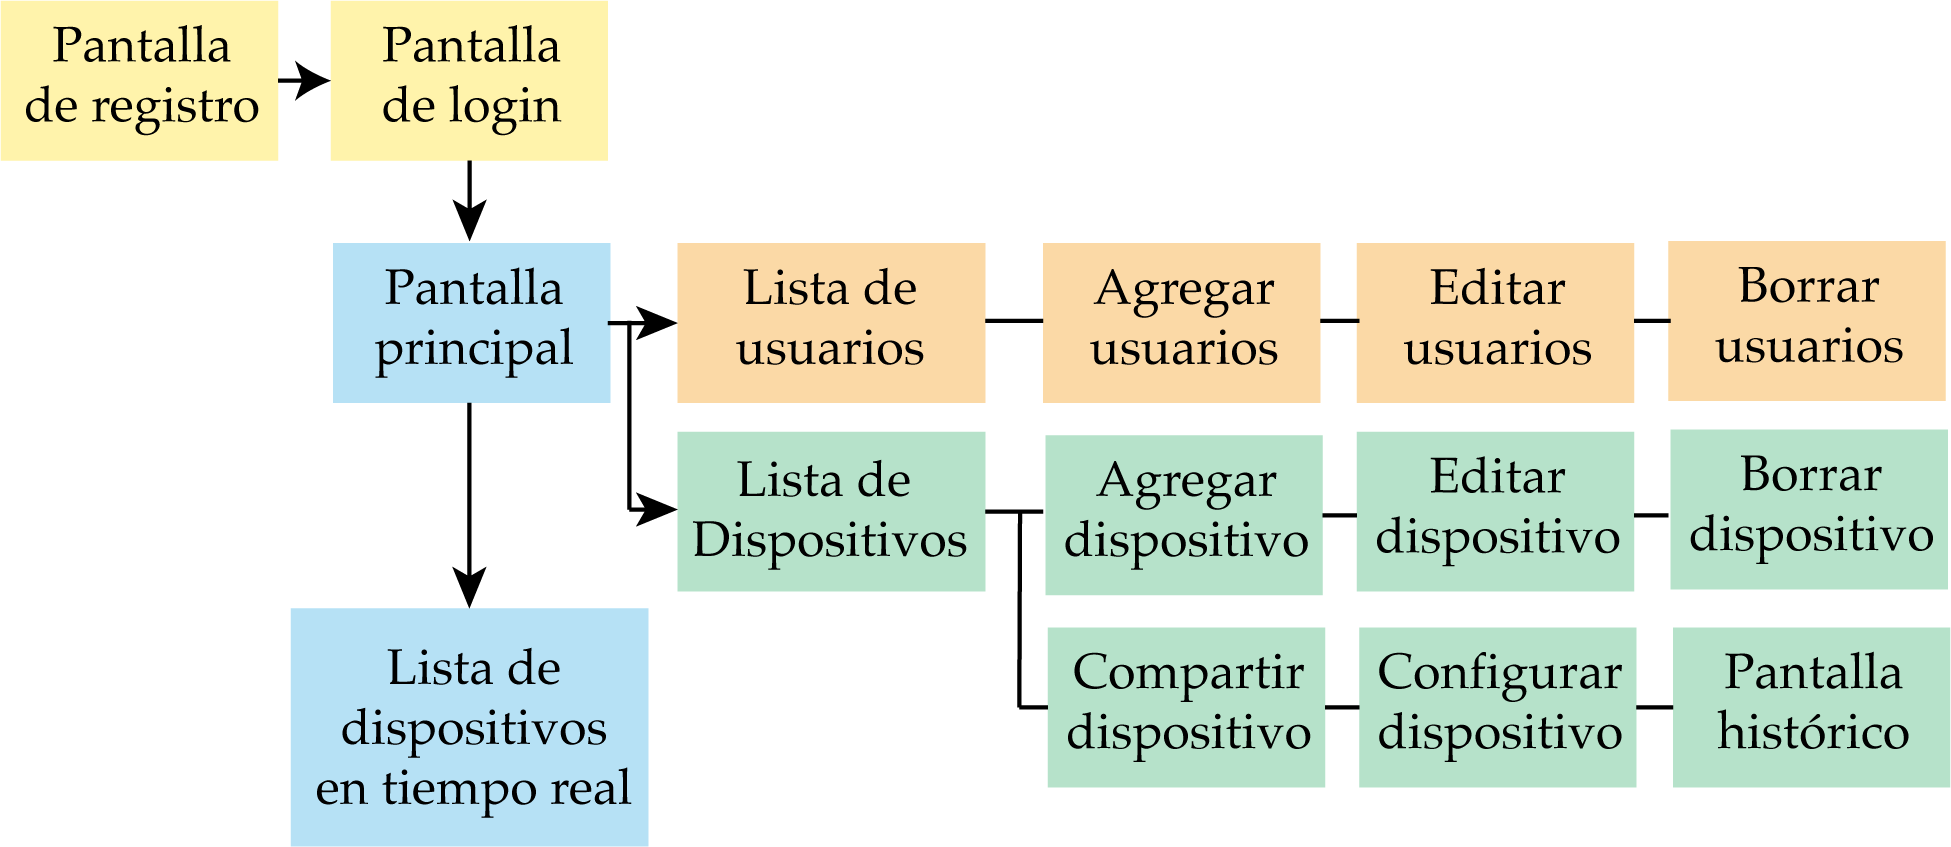
\includegraphics[scale=.75]{./Figures/bloques-pantallas.png}
	\caption[Rutas del sistema]{Ilustración de bloques con rutas implementadas en el sistema.}
	\label{fig:bloque-pantallas}
\end{figure}

Cuando un usuario se registra a la plataforma, por defecto es un usuario administrador. Este rol le permite acceder y crear nuevos usuarios donde puede asignar roles de operador. 

El rol operador, solo permite a los usuarios visualizar información referida a los dispositivos conectados, invalidando la posibilidad de editar, borrar o agregar dispositivos y usuarios.


En la pantalla principal o también llamada \textit{dashboard}, se muestran dispositivos que se encuentran agregados al sistema por parte de un usuario administrador. Estos, son leídos desde la base de datos cuando el usuario ingresa a la plataforma y se adaptan a un modelo de sensor cargado en el sistema. En la figura \ref{fig:dashboard} se muestran dos dispositivos que hacen referencia a sensores de temperatura fabricados por la empresa D\&T que utilizan el modulo conversor Modbus a MQTT.
\pagebreak
 \begin{figure}[htpb]
	\centering
	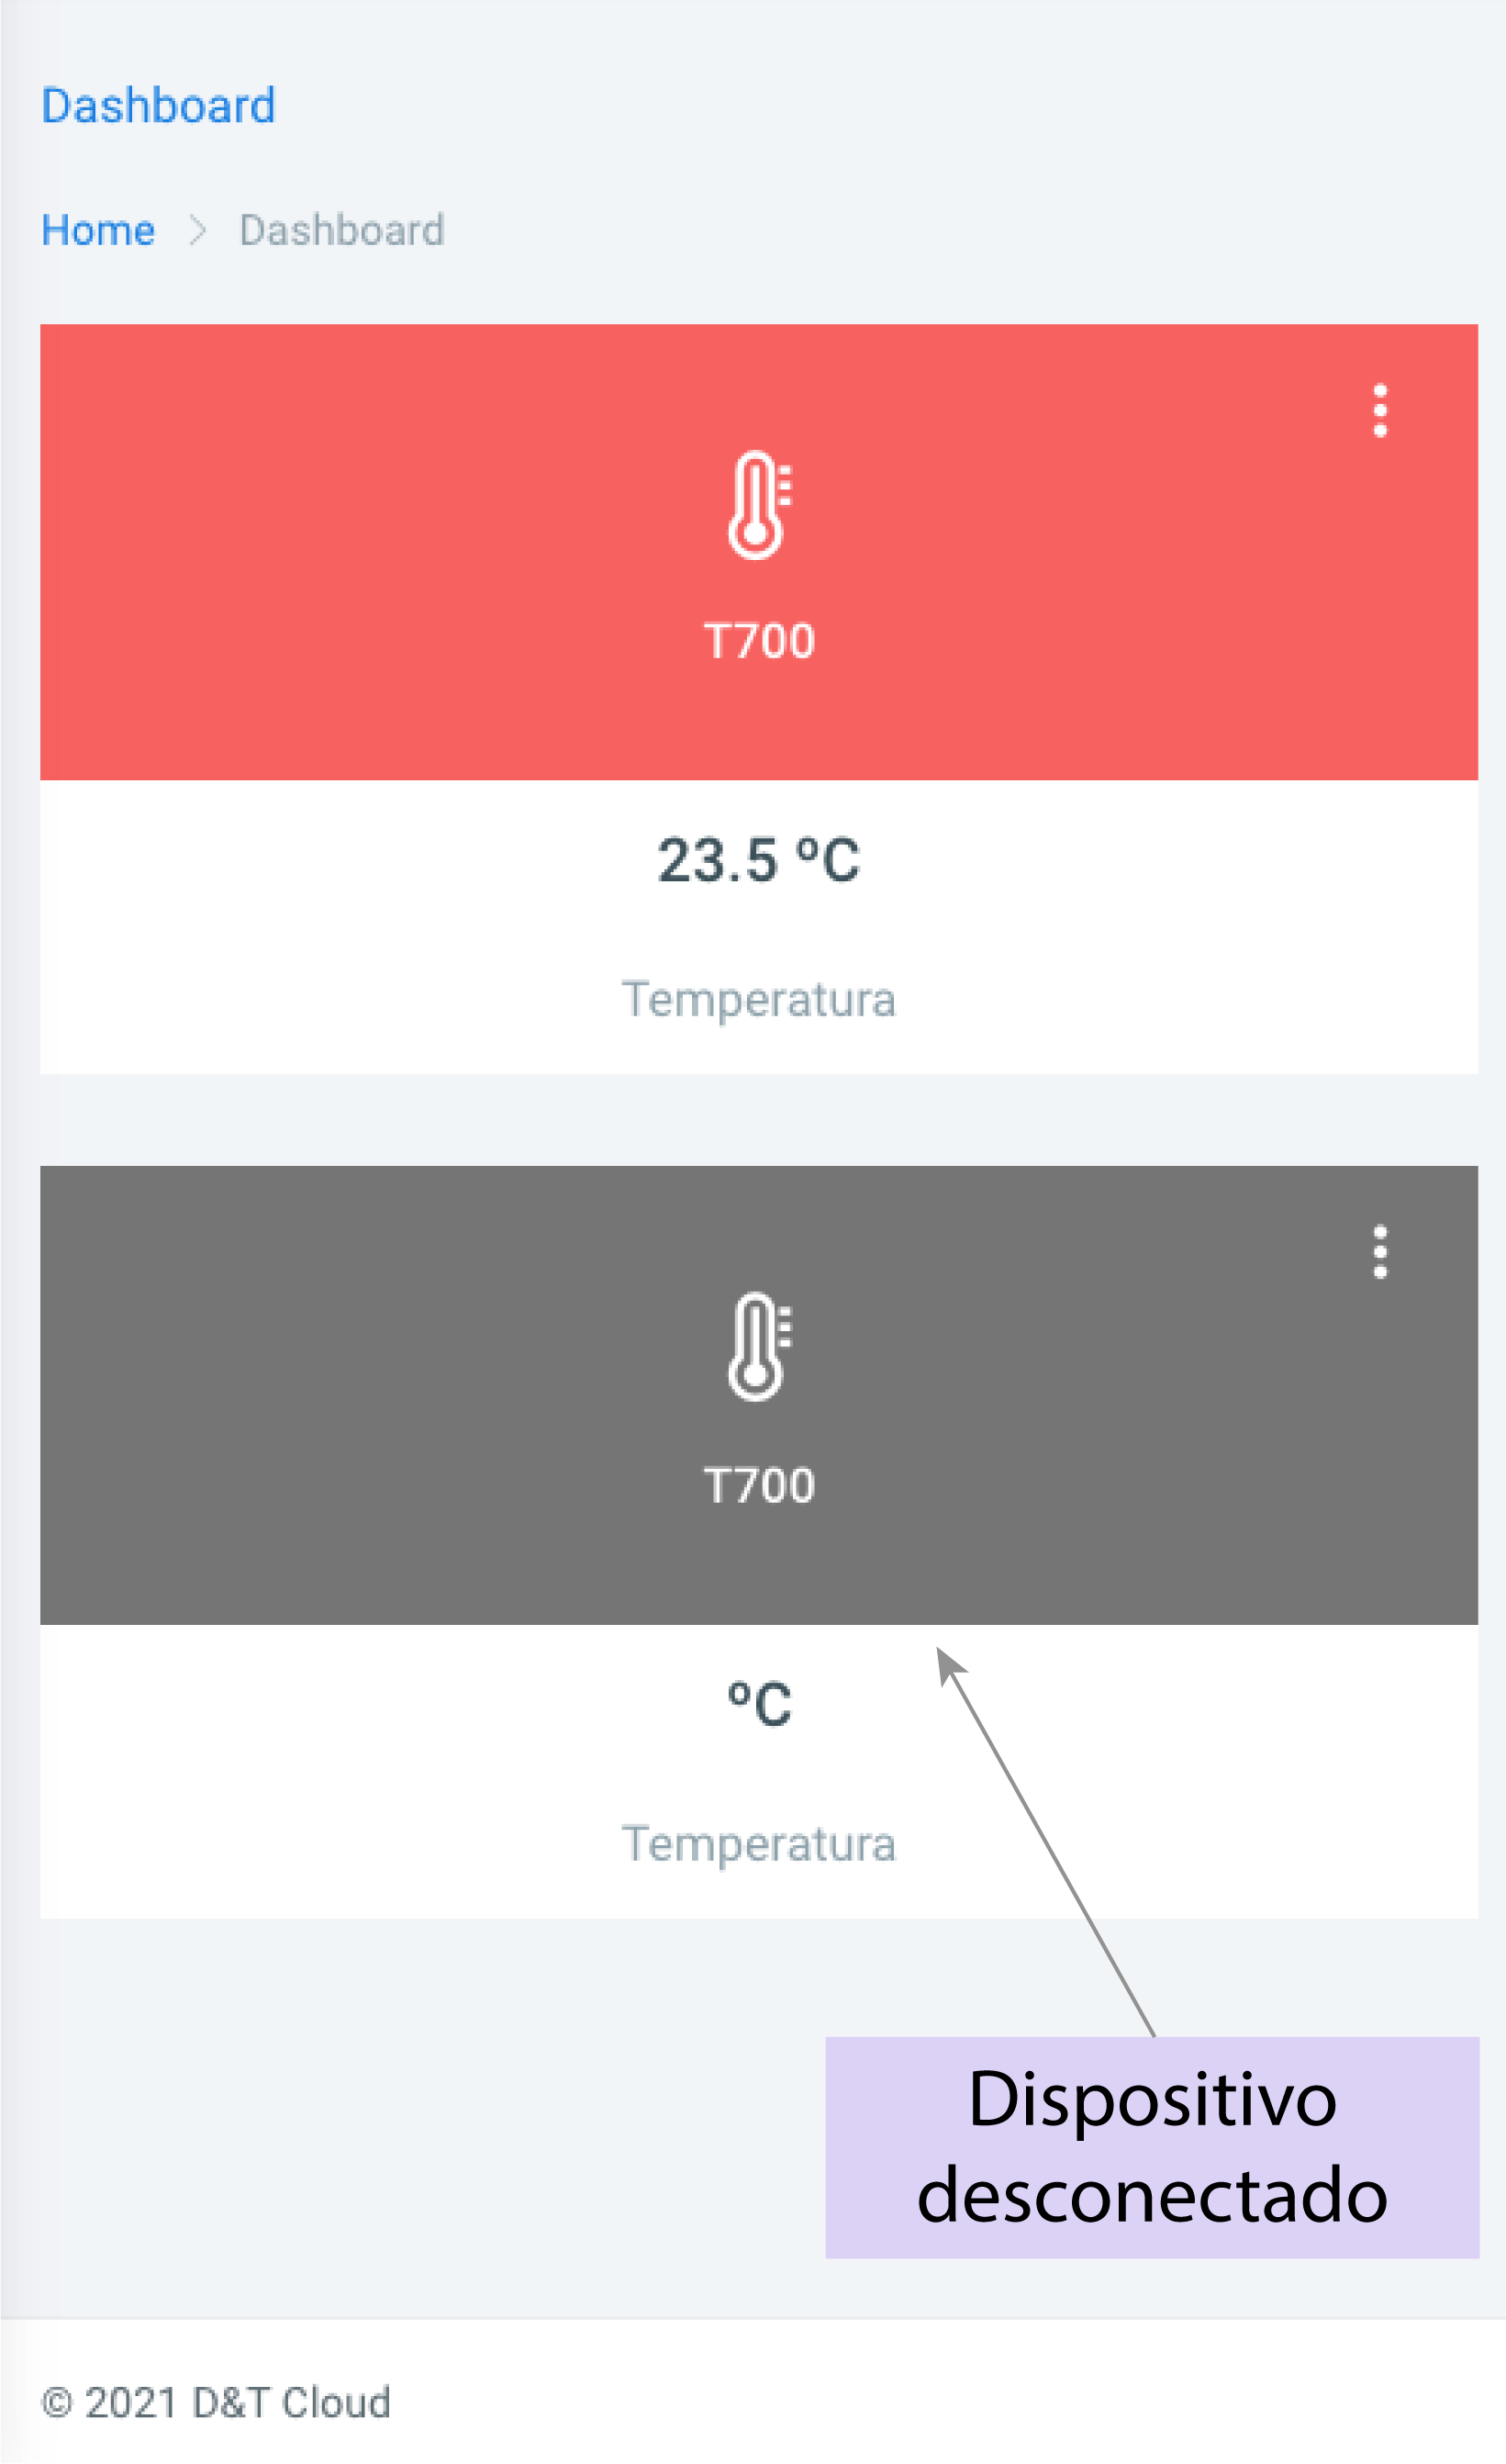
\includegraphics[scale=.7]{./Figures/dashboard.png}
	\caption[Pantalla principal - \textit{dashboard}]{Ilustración de lista de sensores de temperatura T700 conectados a conversores Modbus a MQTT. }
	\label{fig:dashboard}
\end{figure}



Cada bloque de sensor corresponde a un componente de Angular, el cual tiene un servicio asociado para el manejo de datos en tiempo real y además la posibilidad de acceder a sus datos históricos. En la figura \ref{fig:sensor-temp} se observa en detalle las opciones de acceso implementadas en el componente.
\pagebreak
 \begin{figure}[htpb]
	\centering
	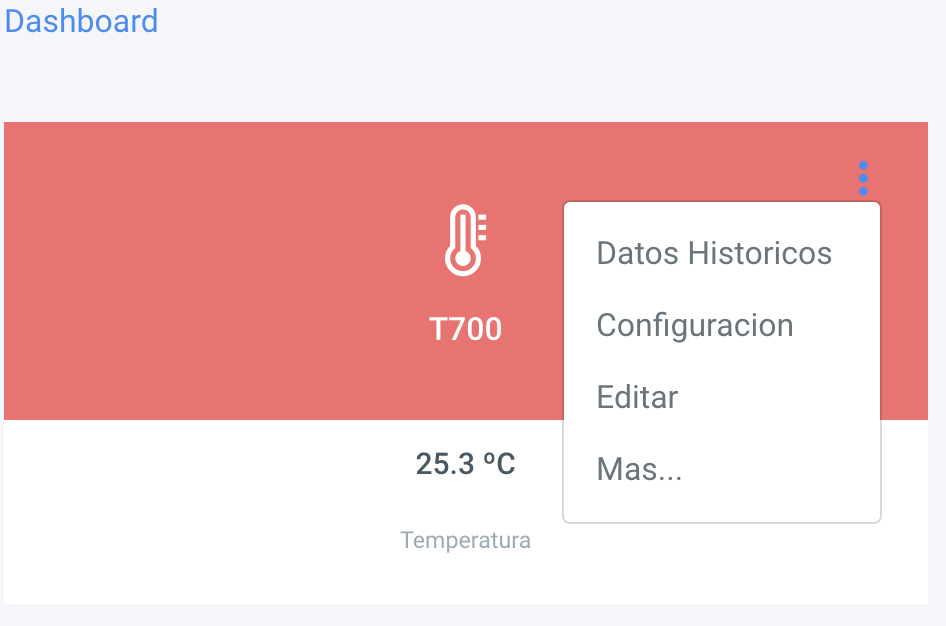
\includegraphics[scale=.60]{./Figures/sensor-temp.png}
	\caption[Sensor de temperatura T700]{Ilustración de componente utilizado para modelar el sensor T700 y sus opciones de acceso.}
	\label{fig:sensor-temp}
\end{figure}


Si el usuario requiere realizar cambios en el dispositivo y editar parámetros como se muestra en la figura \ref{fig:edicion-dev}, puede ingresar directamente desde el componente y sus accesos directos, o bien buscarlo en el listado de dispositivos y presionando en el botón de edición.
\pagebreak
 \begin{figure}[htpb]
	\centering
	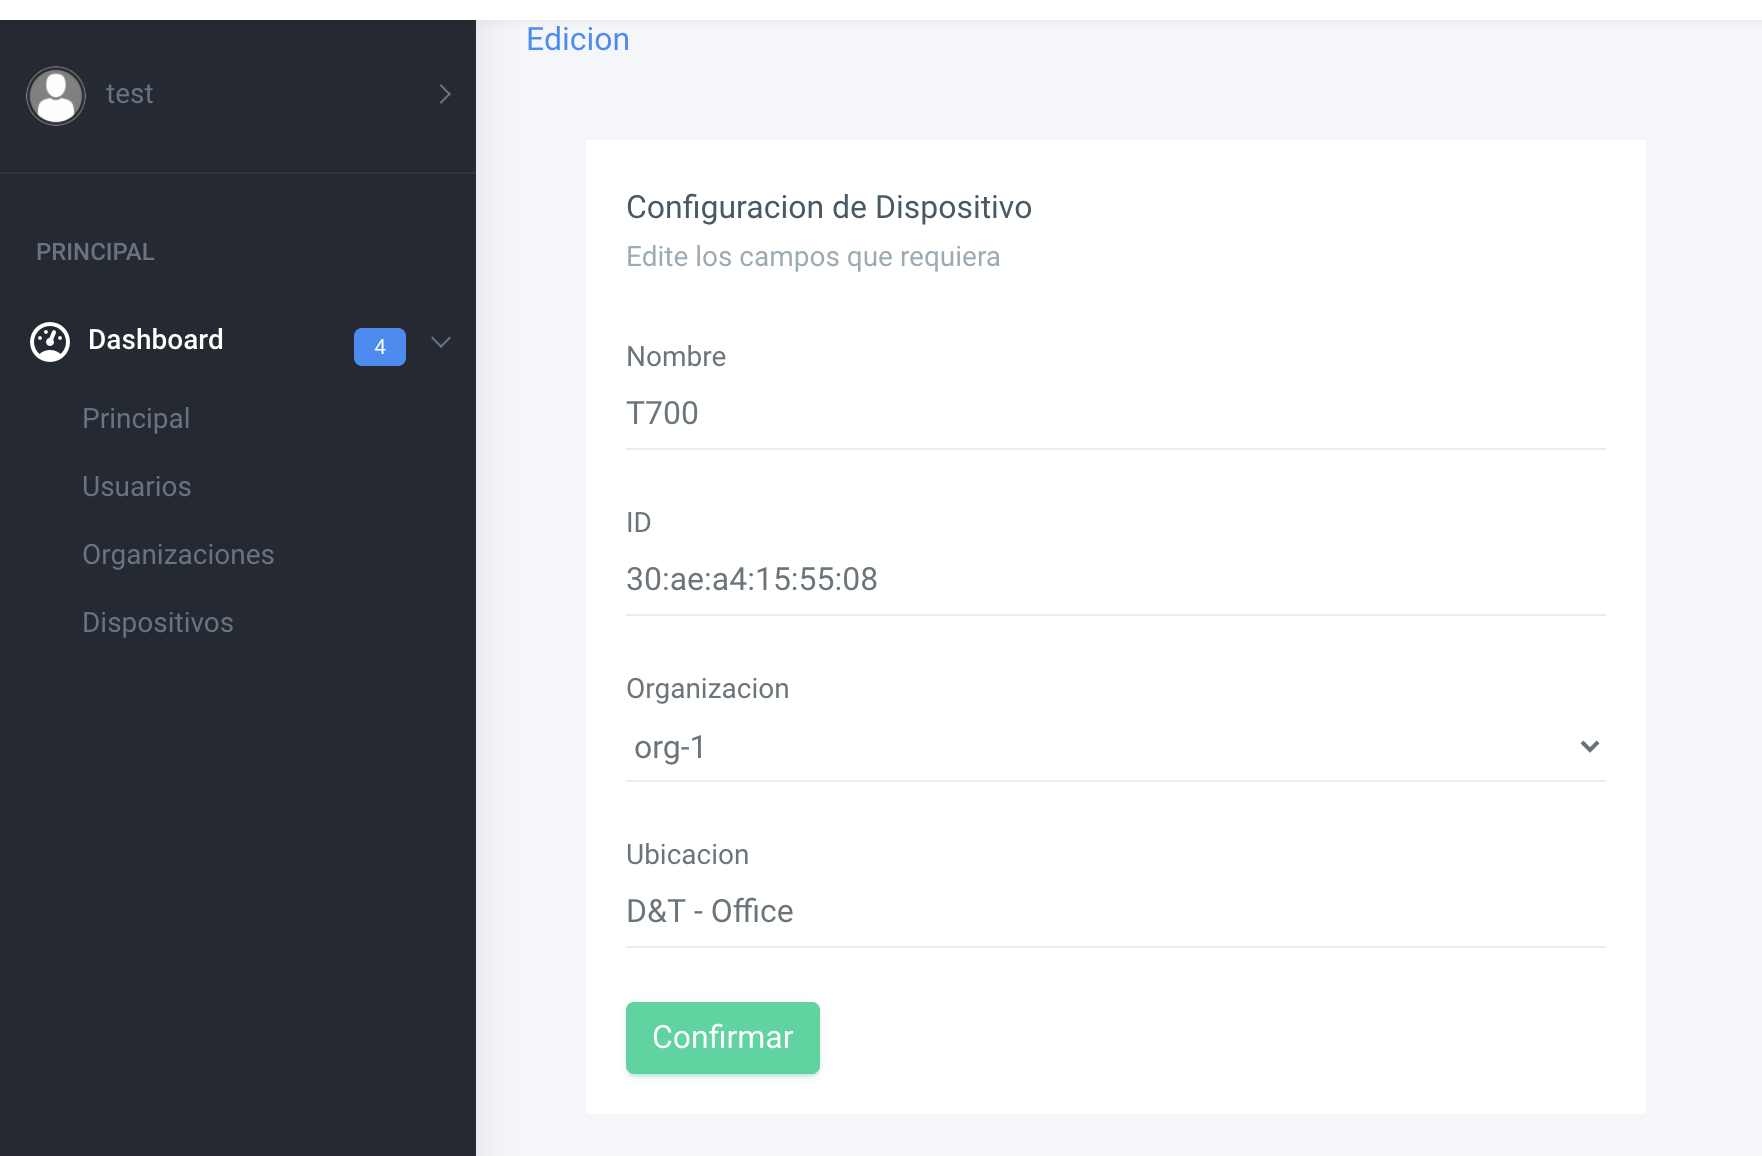
\includegraphics[scale=.55]{./Figures/edicion-dev.png}
	\caption[Pantalla de edición de dispositivos]{Ilustración de pantalla de edición de dispositivos.}
	\label{fig:edicion-dev}
\end{figure}


Para la visualización de datos históricos de dispositivos se utilizó la librería para Angular echarts \citep{WEBSITE:43}. Esta amplia librería permite la utilización de gráficos para mostrar datos históricos de mediciones de los dispositivos que almacenan datos en MongoDB. En la figura \ref{fig:echart-grafica} puede observarse las características principales que ofrece el componente para realizar un gráfico y las opciones correspondientes en la figura \ref{fig:echart-grafica-opciones}.

\begin{figure}[htpb]
	\centering
	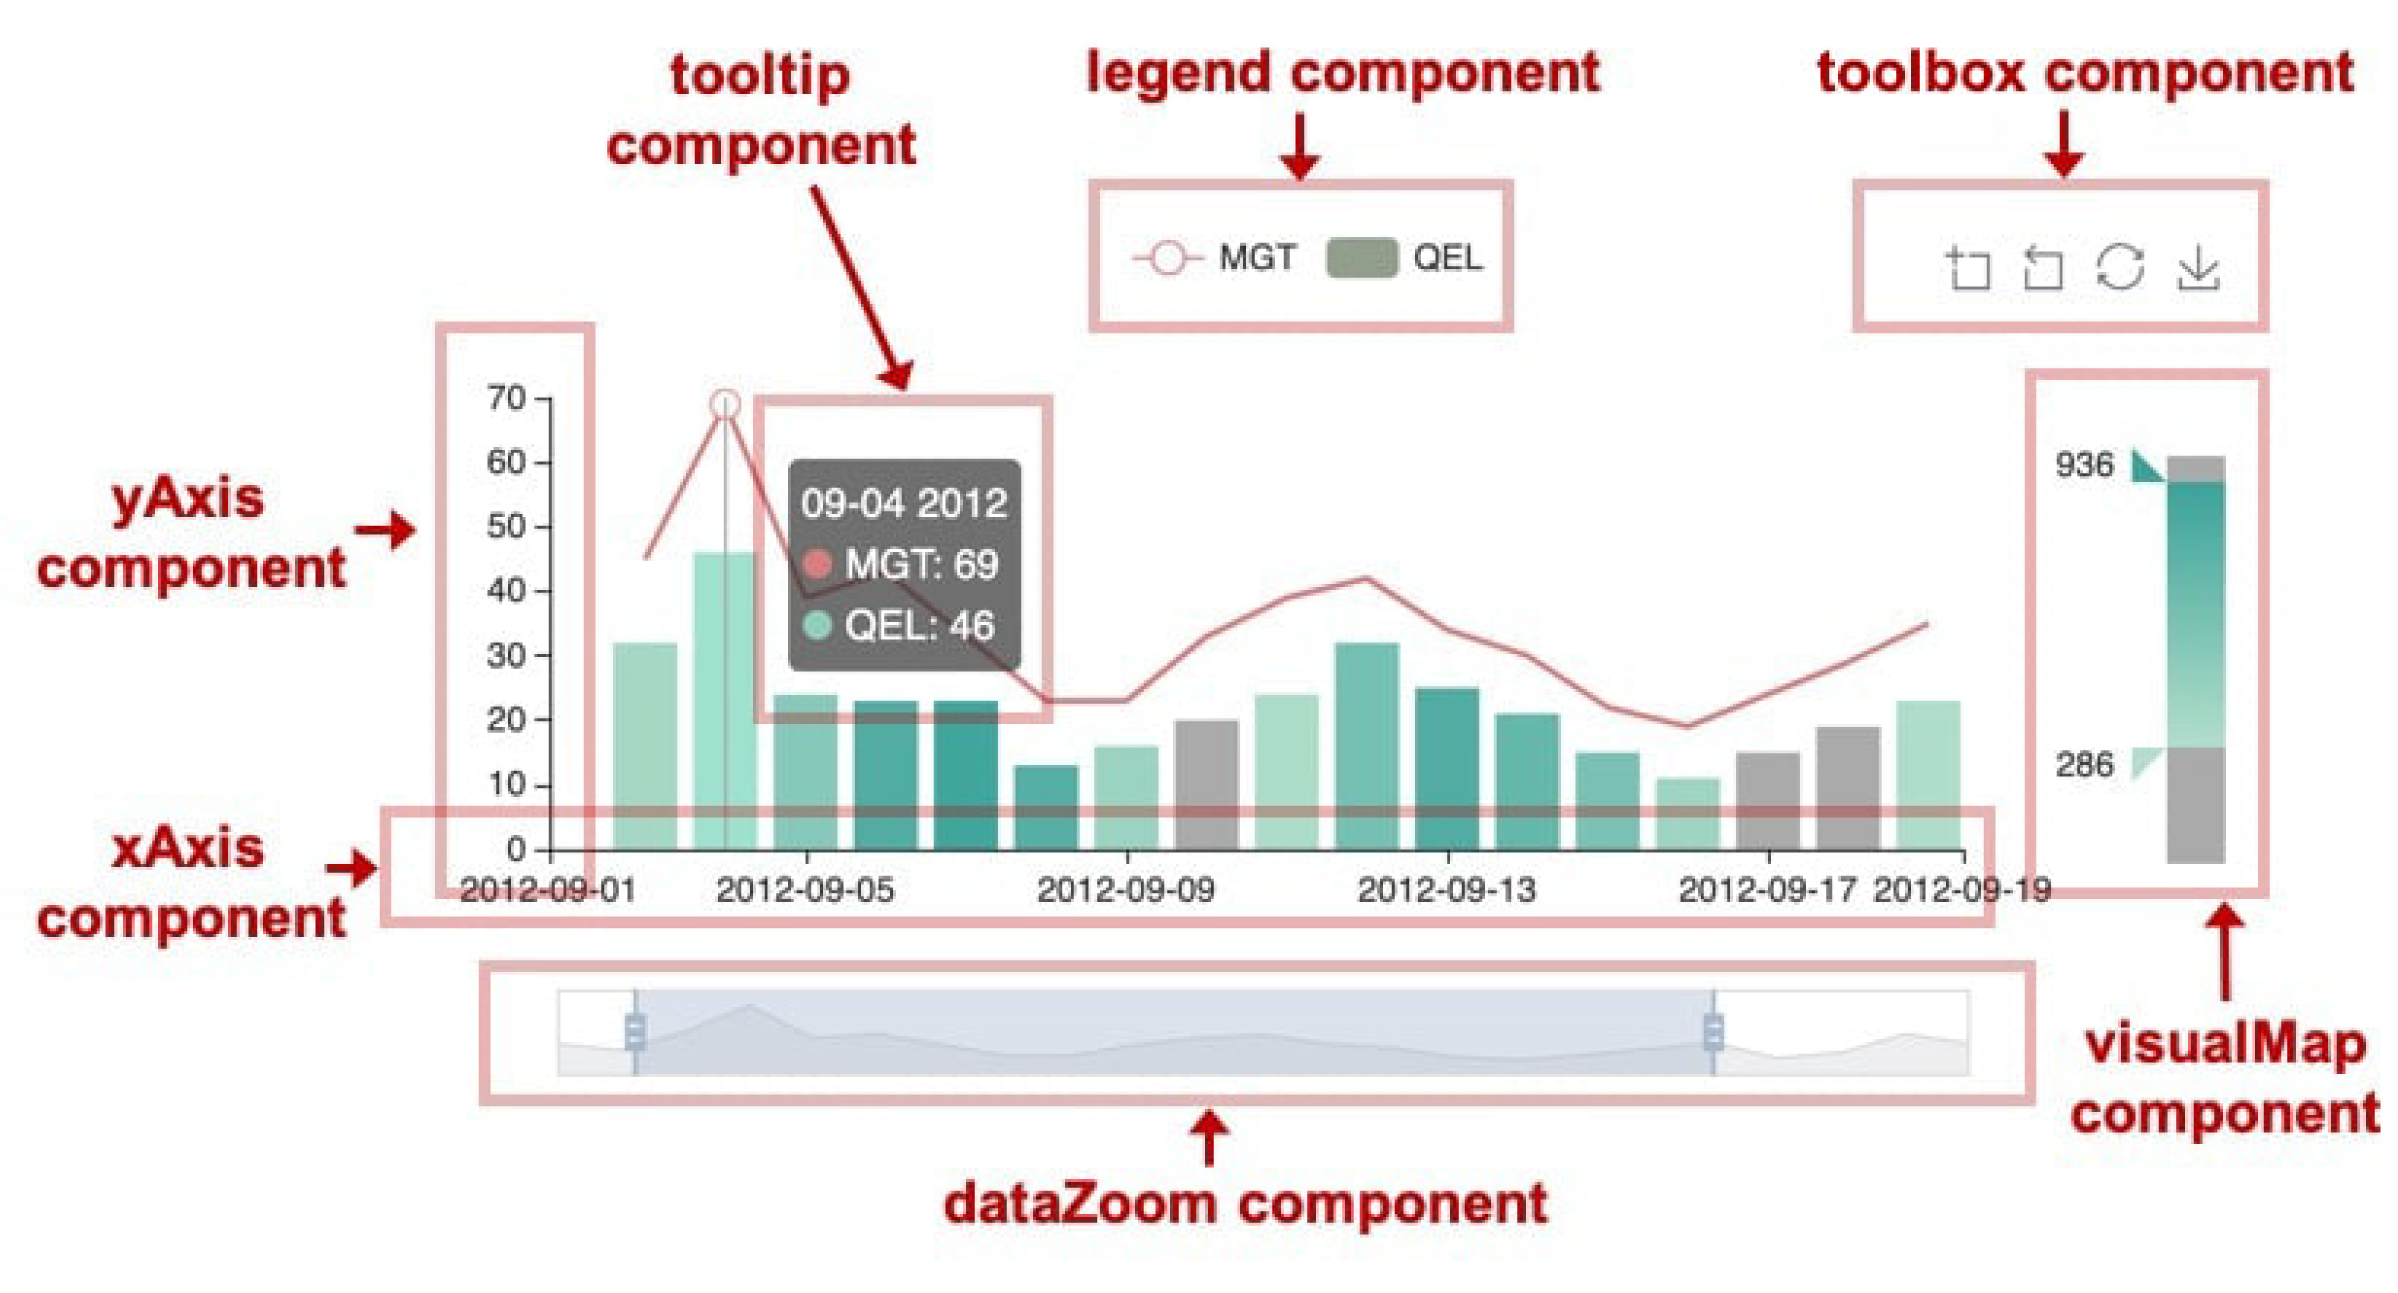
\includegraphics[scale=.60]{./Figures/echart-grafica.png}
	\caption[Componente gráfico de echarts]{Ilustración de componente gráfico utilizando la librería echart\protect\footnotemark.}
	\label{fig:echart-grafica}
\end{figure}


\footnotetext{Fragmento de imagen tomada de \url{https://echarts.apache.org/en/tutorial.html}}



\begin{figure}[htpb]
	\centering
	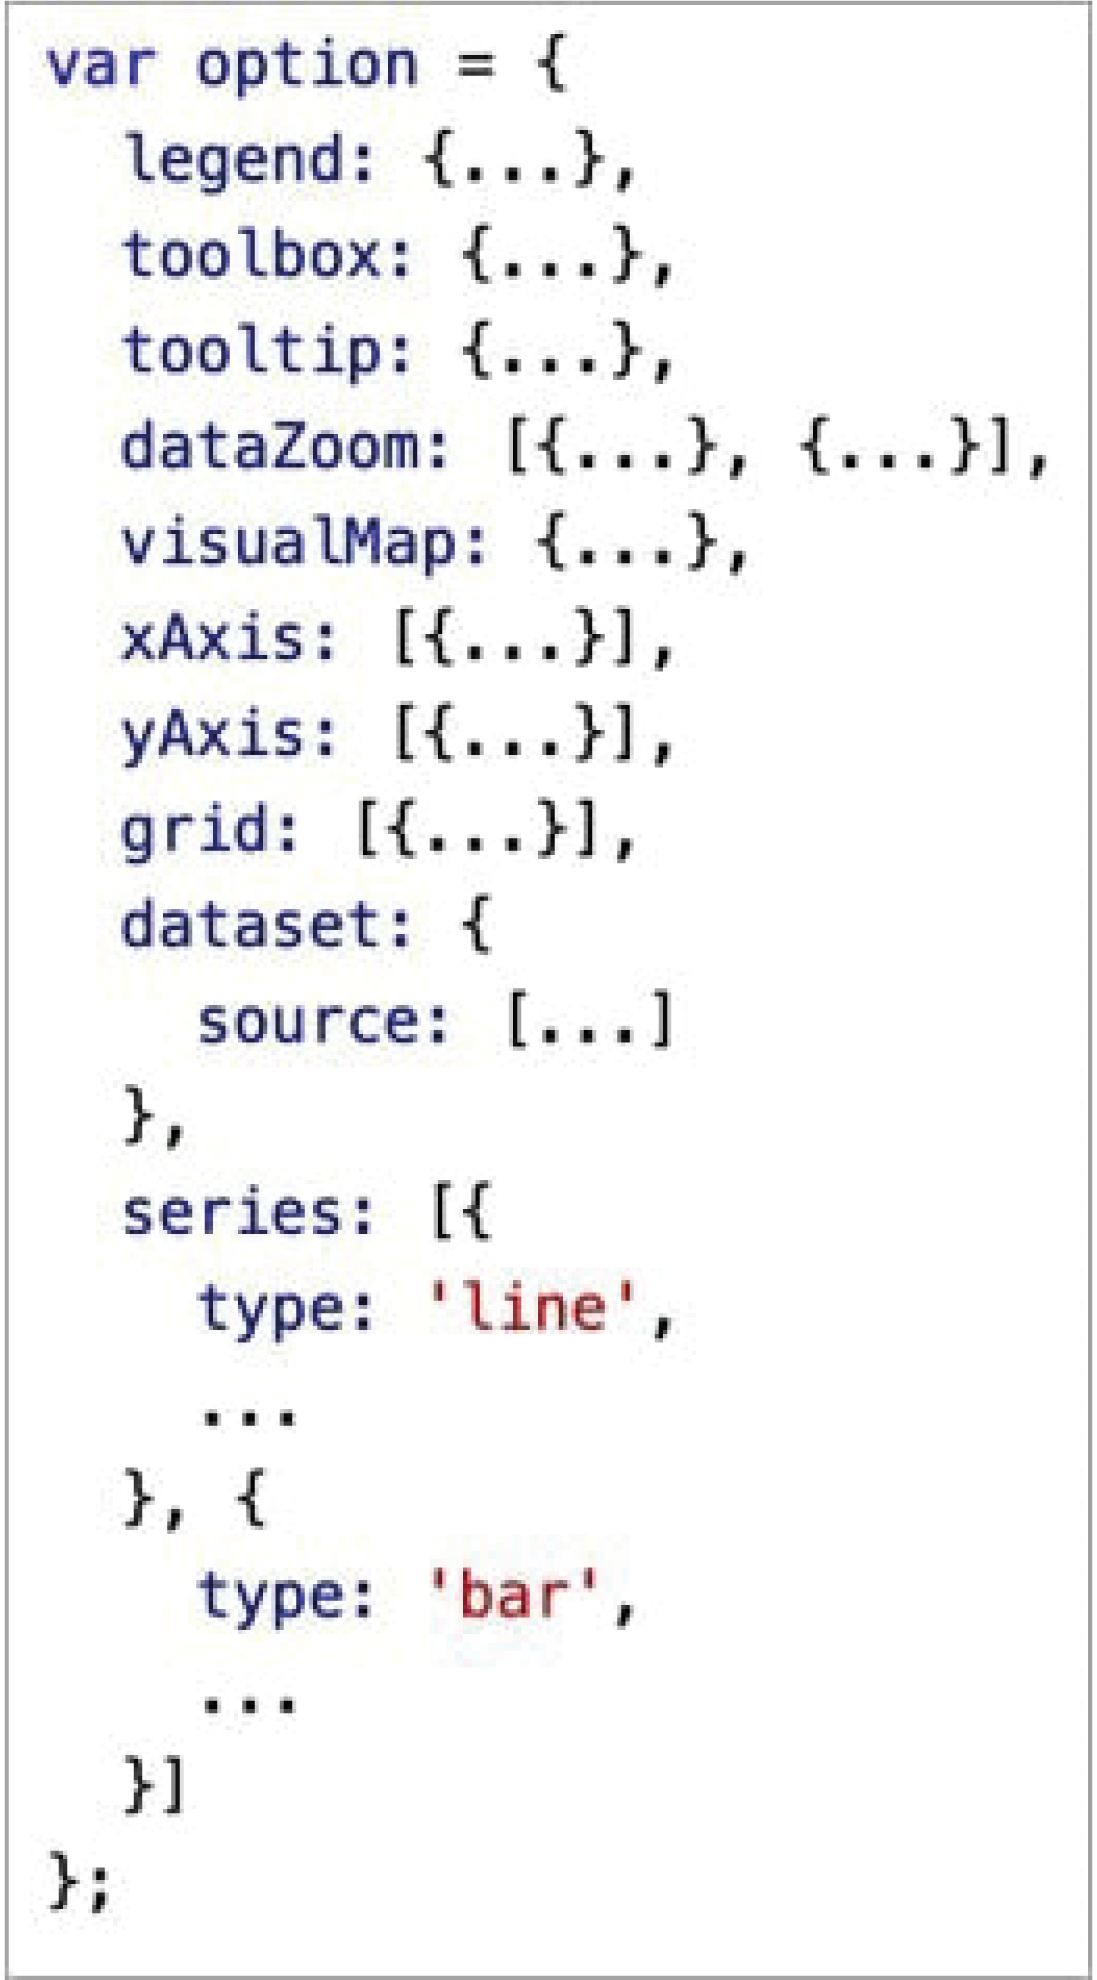
\includegraphics[scale=.60]{./Figures/echart-grafica-options.png}
	\caption[Opciones de configuración de echarts]{Ilustración de opciones de configuración de gráfico utilizando echarts\protect\footnotemark.}
	\label{fig:echart-grafica-opciones}
\end{figure}

\footnotetext{Fragmento de imagen tomada de \url{https://echarts.apache.org/en/tutorial.html}}


\newpage

La figura \ref{fig:device-grafica} muestra el gráfico de mediciones históricas que corresponden a un sensor de temperatura que utiliza un dispositivo conversor de datos Modbus a MQTT.


\begin{figure}[htpb]
	\centering
	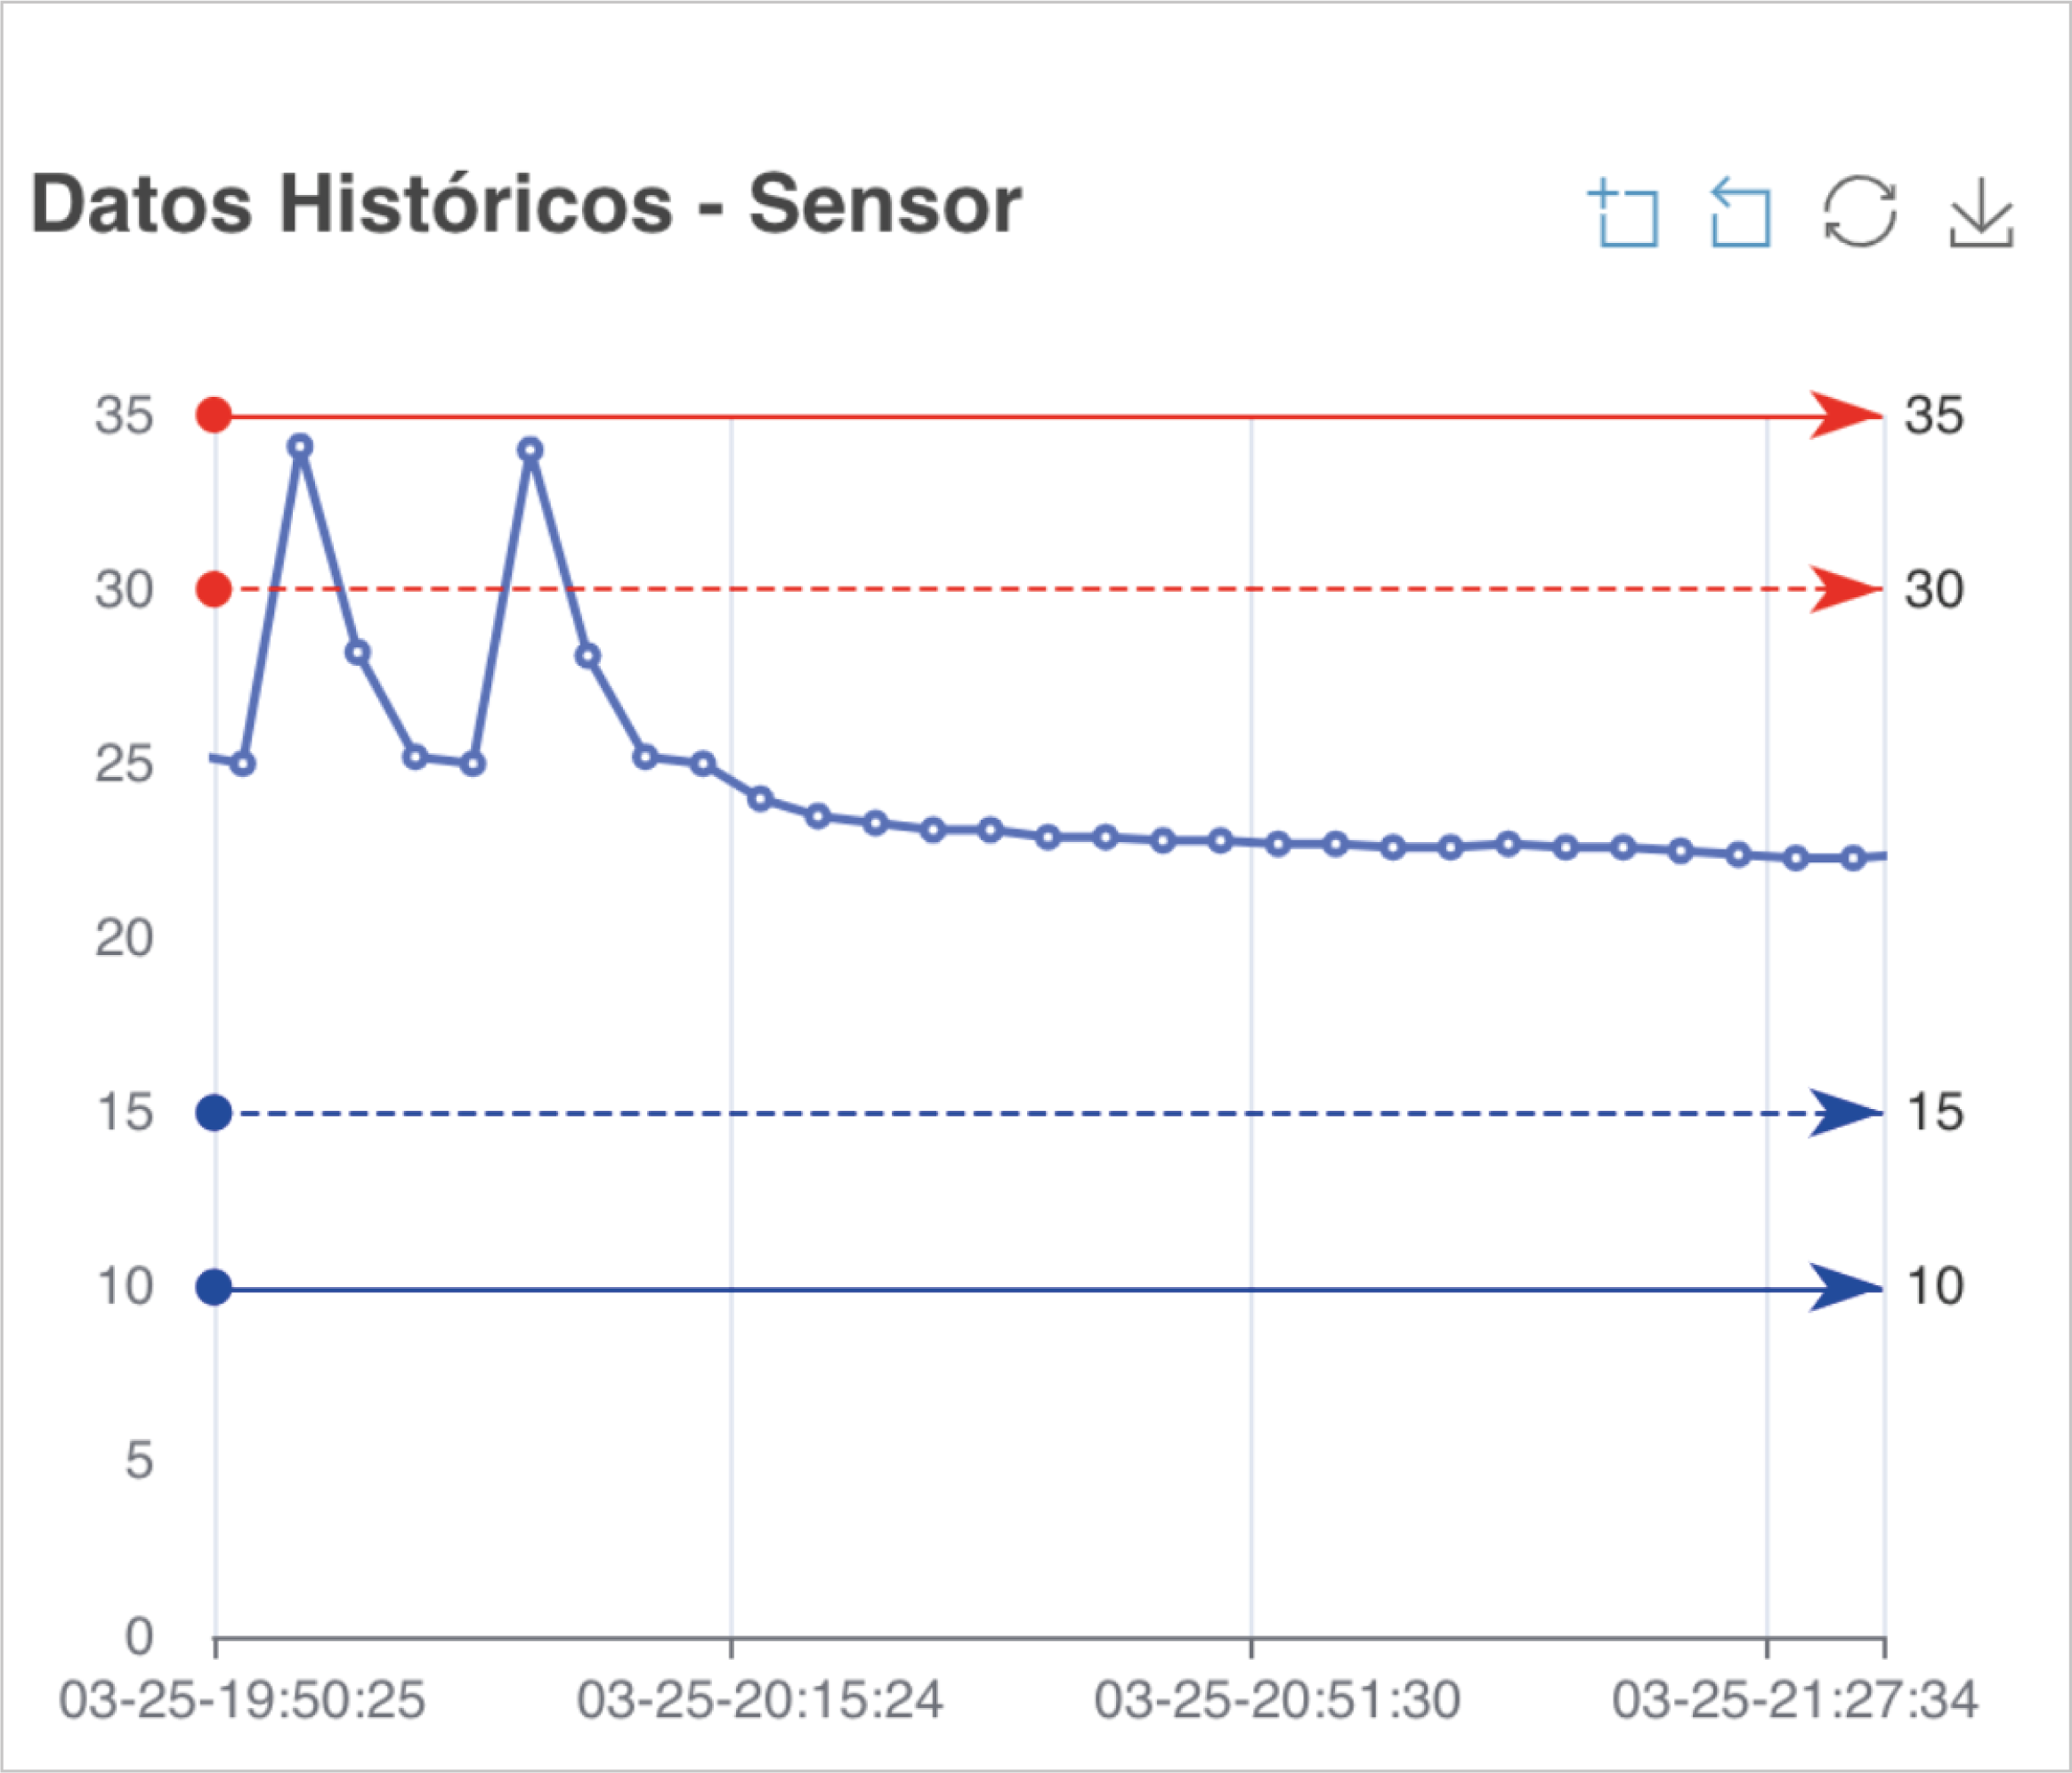
\includegraphics[scale=.65]{./Figures/device-grafica.png}
	\caption[Componente gráfico de echarts]{Ilustración de datos históricos de sensor de temperatura conectado a conversor de datos Modbus a MQTT.}
	\label{fig:device-grafica}
\end{figure}


El diseño web \textit{responsive} o adaptativo es una técnica de diseño web que busca la correcta visualización de una misma página en distintos dispositivos. Desde computadoras de escritorio a tablets y móviles.  Se trata de dimensionar y colocar los elementos de la web de forma que se adapten al ancho de cada dispositivo, permitiendo una correcta visualización y una mejor experiencia de usuario.  Para el diseño de la plataforma se utilizaron componentes con estilos que se adaptan a diferentes tamaños de pantallas. 


En la figura \ref{fig:pantalla-pc}. se observa la visualización de la pantalla principal adaptada para pantallas que son utilizadas en PC de escritorio, se debe notar que el usuario puede visualizar el contenido completo, teniendo en cuenta la barra lateral desplegada con las opciones disponibles. 
\pagebreak
\begin{figure}[htpb]
	\centering
	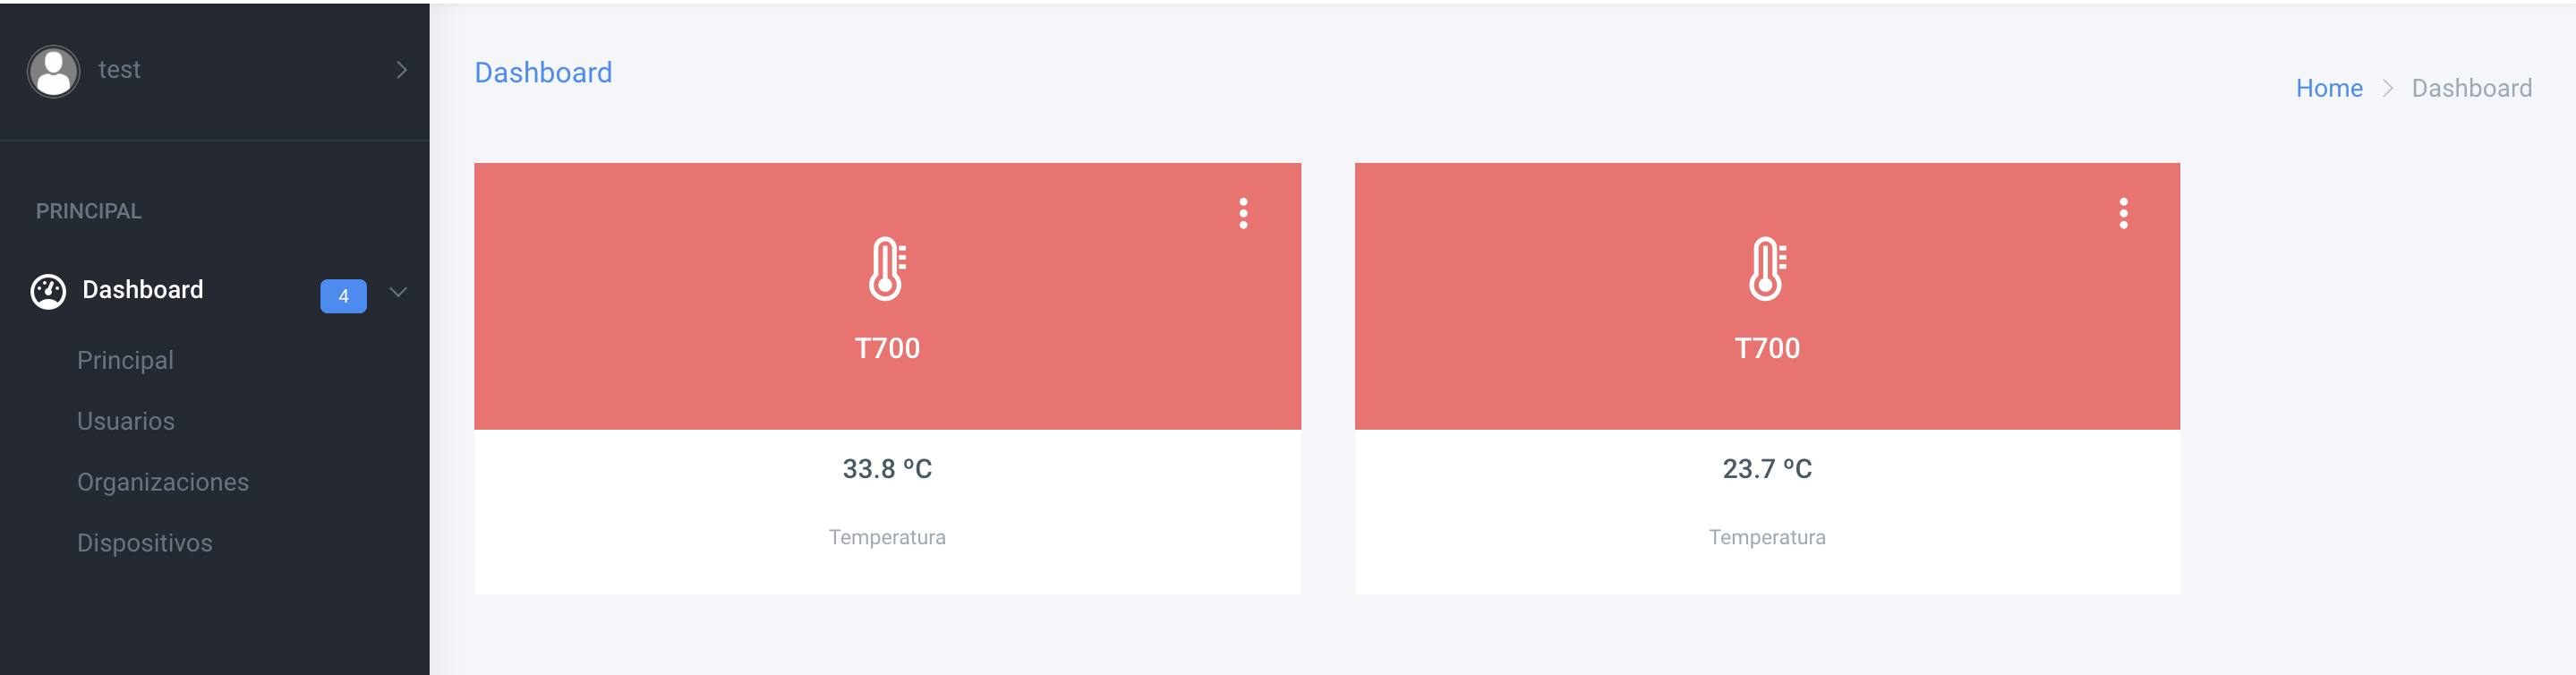
\includegraphics[scale=.68]{./Figures/pantalla-pc.png}
	\caption[Pantalla adaptada a pantallas para PC]{Ilustración de pantalla principal adaptada a pantallas de PC.}
	\label{fig:pantalla-pc}
\end{figure}



Por otro lado la figura \ref{fig:pantalla-tablet} muestra la pantalla adaptada a tablets y que se encuentran de forma horizontal, donde se aprecia que la barra lateral se oculta y si el usuario necesita algún item deberá presionar el botón correspondiente para poder desplegarla. 

\begin{figure}[htpb]
	\centering
	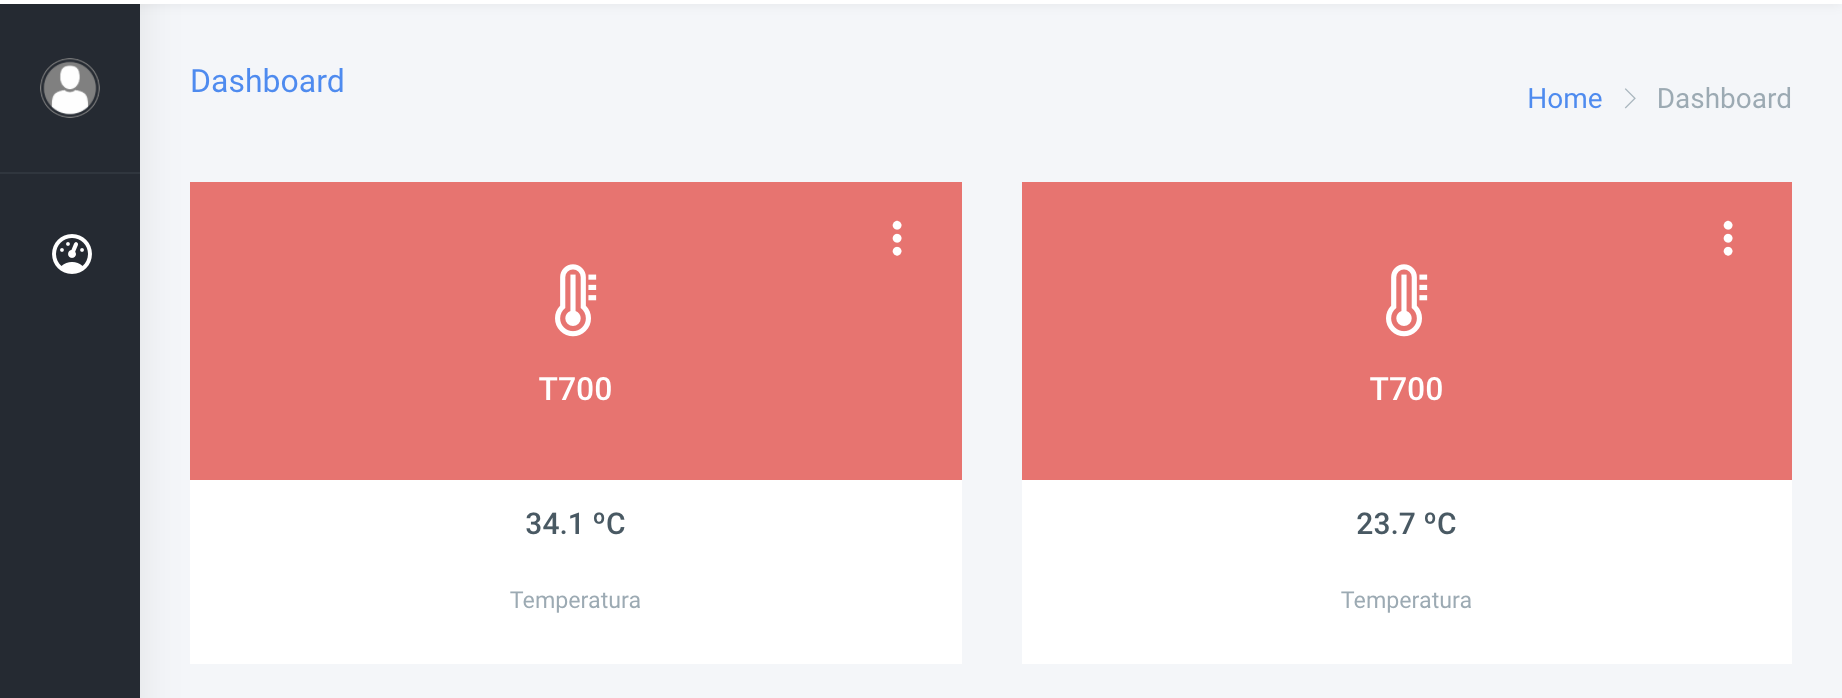
\includegraphics[scale=.55]{./Figures/pantalla-tablet.png}
	\caption[Pantalla adaptada a tablets]{Ilustración de pantalla principal adaptada a tablets.}
	\label{fig:pantalla-tablet}
\end{figure}

\pagebreak
En ultima instancia, la figura \ref{fig:pantalla-celu} muestra la pantalla adaptada para celulares y se aprecia el listado de dispositivos en sola columna y la barra lateral oculta para poder desplegarla a través de un botón.

\begin{figure}[htpb]
	\centering
	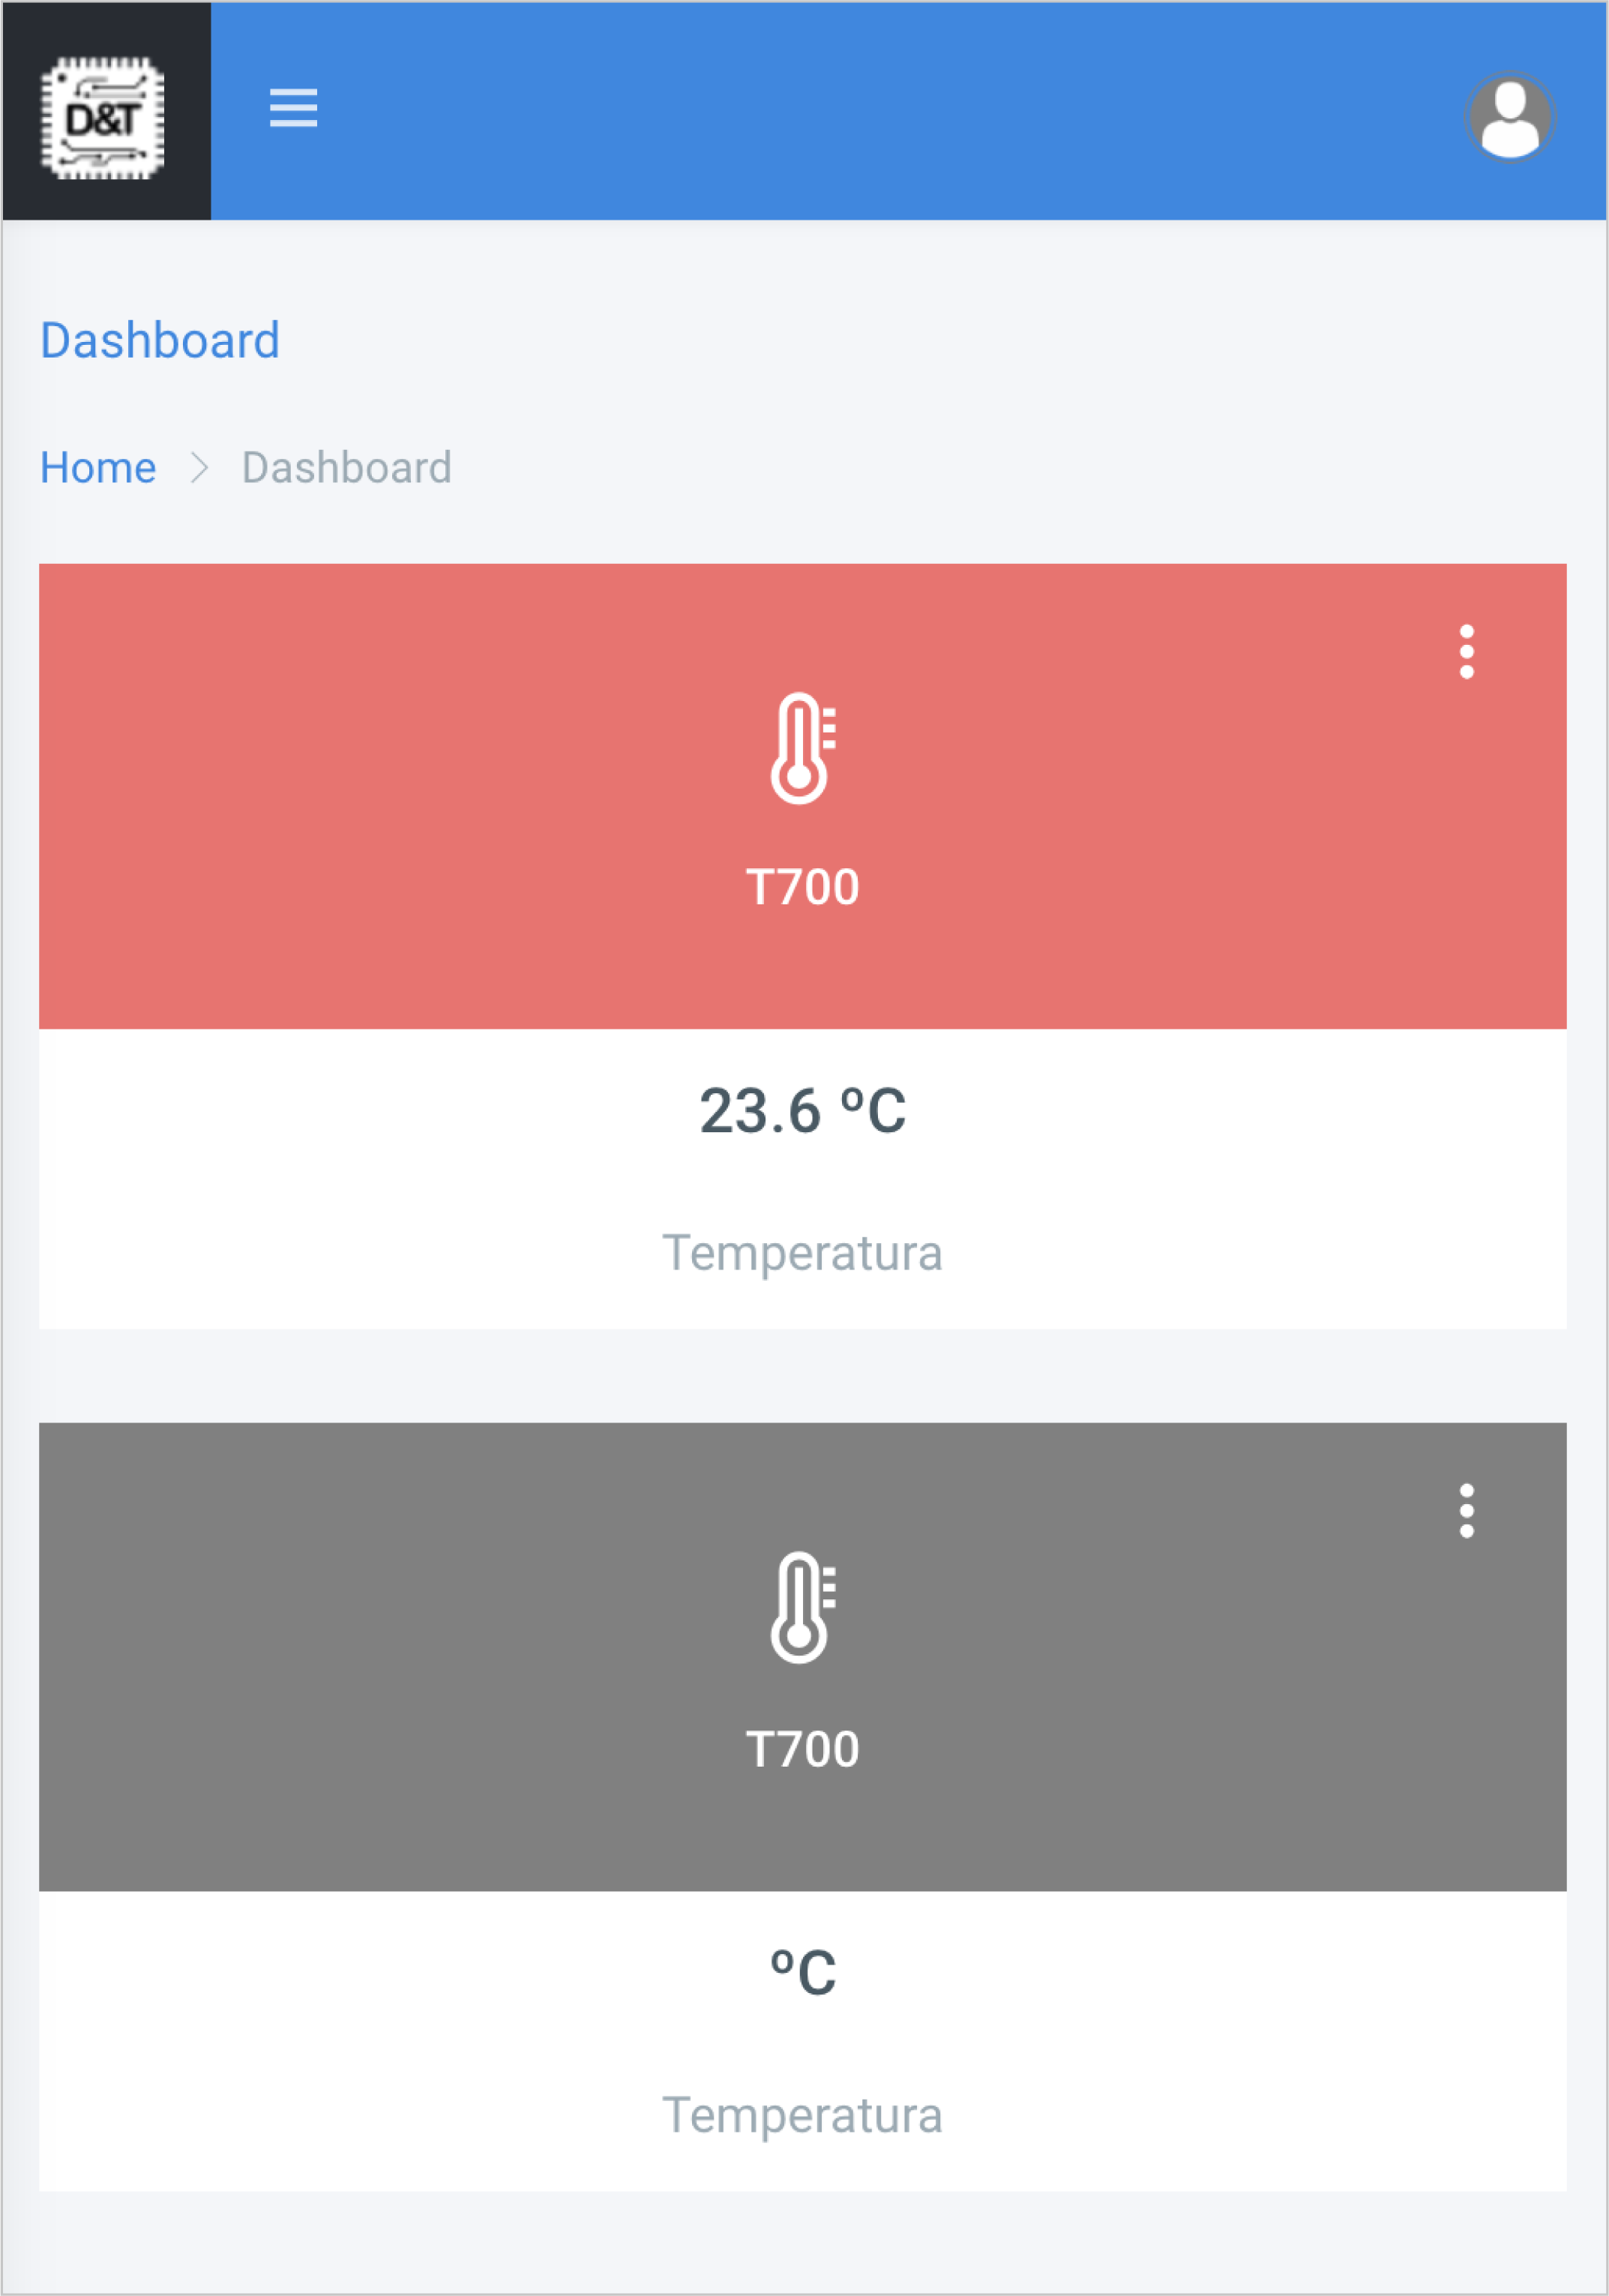
\includegraphics[scale=.60]{./Figures/pantalla-celu.png}
	\caption[Pantalla adaptada a celulares]{Ilustración de pantalla principal adaptada a celulares.}
	\label{fig:pantalla-celu}
\end{figure}

\newpage
\section{Implementación y configuración de Nginx}

Para implementar Nginx en un servidor con sistema operativo Linux como el de este trabajo,  se debe instalarlo con el comando que se muestra en el código \ref{cod:nginx-install}. 

\begin{lstlisting}[label=cod:nginx-install,caption=Instalación de Nginx en servidor con sistema operativo Linux.] 

// Instalacion de Nginx
sudo apt install nginx

// Aplicar ajustes al firewall

sudo ufw app list

sudo ufw allow 'Nginx HTTP'

// Comprobar que Nginx funcione en el servidor
systemctl status nginx

\end{lstlisting} 

Para la configuración de Nginx en el servidor se deben tener en cuenta los siguientes archivos y directorios y como cada uno influye en el funcionamiento:

\begin{itemize}
	\item /etc/nginx: directorio de configuración de Nginx. En él se encuentran todos los archivos de configuración de Nginx.
	
	\item /etc/nginx/nginx.conf: archivo de configuración principal de Nginx. Esto se puede modificar para realizar cambios en la configuración general de Nginx.
	
	\item /etc/nginx/sites-available/: directorio en el que se pueden guardar bloques de servidor por sitio. Nginx no utilizará los archivos de configuración de este directorio a menos que estén vinculados al directorio sites-enabled. Normalmente, toda la configuración del bloque de servidor se realiza en este directorio y luego se habilita estableciendo un vínculo con el otro directorio.
	
	\item /etc/nginx/sites-enabled/: directorio en el que se almacenan los bloques de servidor habilitados por sitio. Normalmente, estos se crean estableciendo vínculos con los archivos de configuración del directorio sites-available.

	\item /etc/nginx/snippets: este directorio contiene fragmentos de configuración que pueden incluirse en otras partes de la configuración de Nginx. Los segmentos de configuración potencialmente repetibles reúnen las condiciones para la conversión a fragmentos.
\end{itemize}

Los dominios utilizados para este trabajo son:

\begin{itemize}
	\item frontend: \url{https://cloud.dytsoluciones.com.ar}.
	
	\item backend: \url{https://api.cloud.dytsoluciones.com.ar}.
\end{itemize}

La configuración para el frontend se realizó siguiendo los pasos del código \ref{cod:nginx-config}.

\begin{lstlisting}[label=cod:nginx-config,caption=Configuración de Nginx en servidor con sistema operativo Linux.] 

// Se crea el directorio con el nombre de dominio utilizado
sudo mkdir -p /var/www/cloud.dytsoluciones.com.ar/html

//Se asigna la propiedad del directorio con la variable de entorno $USER
sudo chown -R $USER:$USER /var/www/cloud.dytsoluciones.com.ar/html

// Para que Nginx pueda utilizar las directivas correcctas se crea un archivo de configuracion predeterminado. 

sudo nano /etc/nginx/sites-available/cloud.dytsoluciones.com.ar

// Se crea el enlace entre el archivo de configuracion y el directorio sites-enabled.
sudo ln -s /etc/nginx/sites-available/cloud.dytsoluciones.com.ar/ /etc/nginx/cloud.dytsoluciones.com.ar/

//Una vez finalizada la configuracion se reinicia el servicio
sudo systemctl restart nginx
\end{lstlisting} 

